% В этом шаблоне используется класс spbau-diploma.
\documentclass[14pt]{spbau-diploma}

\usepackage{graphicx}
\usepackage{longtable}
\usepackage{array}
\usepackage{booktabs}
\usepackage{url}
\usepackage{amsmath}
\usepackage{amssymb}
\usepackage{tikz}
\usetikzlibrary{positioning,arrows.meta,shapes.geometric,fit,calc,backgrounds}

\tikzset{
  msarr/.style={-{Latex[length=2.5mm]},thick},
  msbiarr/.style={{Latex[length=2.5mm]}-{Latex[length=2.5mm]},thick},
  block/.style={draw=black,rounded corners=3pt,align=center,minimum height=1.0cm,
                inner sep=4pt,font=\small},
  block2/.style={draw=black,rounded corners=2pt,align=center,minimum height=0.7cm,
                 inner sep=3pt,font=\footnotesize,fill=gray!10},
  state/.style={draw=black,rounded corners=4pt,align=center,minimum height=0.9cm,
                minimum width=2.6cm,font=\footnotesize}
}

\sloppy
\hbadness=10000
\vbadness=10000
\tolerance=2000
\emergencystretch=3em

\begin{document}

\filltitle{ru}{
    chair              = {Факультет прикладных компьютерных наук},
    title              = {Поддержание базы автономных систем\\ на основе данных протокола BGP},
    type               = {master},
    position           = {студента},
    group              = {P4235},
    author             = {Новокшанов Евгений Андреевич},
    supervisorPosition = {научный руководитель},
    supervisor         = {Белявцев И.\,П.},
    reviewerPosition   = {рецензент},
    reviewer           = {--},
    chairHeadPosition  = {--},
    chairHead          = {--},
    university         = {Национальный исследовательский университет ИТМО},
    faculty            = {Факультет прикладных компьютерных наук},
    city               = {Санкт-Петербург},
    year               = {2026}
}

\filltitle{en}{
    university         = {ITMO University},
    faculty            = {Faculty of Applied Computer Science},
    chair              = {Faculty of Applied Computer Science},
    title              = {Maintaining the Autonomous Systems Database Based on BGP Protocol Data},
    author             = {Evgeny Novokshanov},
    supervisorPosition = {supervisor},
    supervisor         = {Ivan Belyavtsev},
    reviewerPosition   = {reviewer},
    reviewer           = {--},
    chairHeadPosition  = {--},
    chairHead          = {--},
    city               = {Saint Petersburg},
    year               = {2026}
}

\maketitle
\tableofcontents

%==============================================================
\section*{ТЕРМИНЫ И ОПРЕДЕЛЕНИЯ}

В настоящей работе используются следующие термины с соответствующими
определениями.

\begin{description}\setlength{\itemsep}{0.2em}
\item[Автономная система (AS)] -- совокупность сетевых префиксов,
управляемых одним административным субъектом и анонсируемых наружу
по единой маршрутной политике; идентифицируется числом ASN
(Autonomous System Number).
\item[BGP (Border Gateway Protocol)] -- протокол обмена маршрутной
информацией между автономными системами, описанный в RFC~4271
\cite{rfc4271}.
\item[BMP (BGP Monitoring Protocol)] -- протокол наблюдения за
состоянием BGP-сеансов и содержимым таблиц маршрутизации
\cite{rfc7854}.
\item[CIDR (Classless Inter-Domain Routing)] -- модель бесклассовой
адресации, в которой принадлежность адреса префиксу описывается парой
«адрес/длина маски» \cite{rfc4632}.
\item[Длиннейшее совпадение префикса (Longest Prefix Match, LPM)] --
задача поиска по IP-адресу префикса наибольшей длины, которому этот
адрес принадлежит.
\item[Полный снимок маршрутов (snapshot)] -- единомоментный набор
действующих BGP-маршрутов, формирующих полное начальное состояние
таблицы.
\item[Поток обновлений (stream)] -- последовательность отдельных
BGP-сообщений типа update/withdraw, изменяющих состояние таблицы
после загрузки начального снимка.
\item[Adaptive Radix Tree (ART)] -- адаптивное префиксное дерево с
переменным размером узлов, описанное в работе Лейса и др.
\cite{leis2013art}.
\item[\texttt{ranger}] -- прежняя внутренняя реализация хранения
префиксных диапазонов, использовавшаяся для построения таблицы
«IP-префикс~$\rightarrow$~ASN» в BIFIT COLLECTOR. В работе
\texttt{ranger} рассматривается как базовый вариант для сравнения с
новым шардированным ART-хранилищем.
\item[GoBGP] -- открытая реализация BGP-демона на языке Go,
предоставляющая внешнее gRPC-API для управления и наблюдения.
\item[gRPC] -- система удалённого вызова процедур поверх HTTP/2,
используемая для взаимодействия микросервиса с GoBGP и с клиентами.
\item[BIFIT MITIGATOR] -- продукт компании, обеспечивающий защиту от
распределённых атак отказа в обслуживании.
\item[BIFIT COLLECTOR] -- продукт для сбора и анализа сетевого
трафика крупного оператора связи.
\item[SLA (Service Level Agreement)] -- соглашение об уровне
обслуживания, фиксирующее количественные требования к качеству работы
сервиса.
\end{description}

%==============================================================

\section*{СПИСОК СОКРАЩЕНИЙ И УСЛОВНЫХ ОБОЗНАЧЕНИЙ}

\begin{description}\setlength{\itemsep}{0.1em}
\item[API] -- application programming interface
\item[ART] -- Adaptive Radix Tree
\item[AS] -- автономная система
\item[ASN] -- Autonomous System Number
\item[BGP] -- Border Gateway Protocol
\item[BMP] -- BGP Monitoring Protocol
\item[CIDR] -- Classless Inter-Domain Routing
\item[CPU] -- центральный процессор (central processing unit)
\item[DDoS] -- distributed denial of service
\item[gRPC] -- gRPC Remote Procedure Calls
\item[IP] -- Internet Protocol
\item[IPv4 / IPv6] -- четвёртая и шестая версии IP
\item[LPM] -- longest prefix match
\item[MP-BGP] -- multiprotocol BGP
\item[MRT] -- multi-threaded routing toolkit (формат дампов)
\item[NLRI] -- network layer reachability information
\item[RIB] -- routing information base
\item[RIS] -- Routing Information Service (RIPE NCC)
\item[SLA] -- service level agreement
\item[ВКР] -- выпускная квалификационная работа
\end{description}

%==============================================================

\section*{ВВЕДЕНИЕ}

\subsection*{Актуальность темы исследования}
\addcontentsline{toc}{subsection}{Актуальность темы исследования}

Современная защита от DDoS-атак, сетевая аналитика и телеметрия
операторских сетей всё чаще опираются на маршрутный контекст адресов.
Главный элемент этого контекста -- принадлежность IP-адреса автономной
системе: по ASN формируются правила фильтрации, выполняется скоринг
источников трафика, анализируются flow-записи и сопоставляются события с
операторской топологией.

Результаты работы внедряются в инфраструктуру продуктов BIFIT
MITIGATOR (защита от DDoS) и BIFIT COLLECTOR (анализ операторского
трафика). Оба продукта должны опираться на одну и ту же таблицу
\textit{IP-префикс~$\rightarrow$~ASN}, выведенную из полной таблицы
маршрутизации BGP; внешние геолокационные справочники с редким
обновлением не подходят для принятия решений в режиме реального времени.
Устаревшее соответствие префиксов и ASN может приводить к ошибкам
фильтрации, некорректной атрибуции источников атаки и расхождению
трактовки одного и того же события между продуктами. До начала работы
логика построения и обновления этой таблицы была встроена в BIFIT
COLLECTOR, а внутреннее хранилище \texttt{ranger} обновлялось по таймеру
полной заменой снимка: потоковое применение одиночных изменений к
in-memory базе не поддерживалось, а BIFIT MITIGATOR не мог
переиспользовать ту же реализацию без дублирования кода и данных.

Естественным первичным источником актуальных данных остаётся сам
протокол BGP~\cite{rfc4271}. Чтобы использовать его в сервисе
сопоставления префиксов и ASN, нужно получить начальный снимок RIB,
непрерывно обрабатывать
update-сообщения, поддерживать IPv4 и IPv6 и подобрать in-memory
структуру, которая одновременно обеспечивает малое время LPM-запроса и
позволяет применять инкрементальные изменения отдельных префиксных
записей без полной перестройки таблицы.

В режимах, где задержка актуализации на уровне нескольких часов не
влияет на прикладное решение, могут применяться внешние справочники.
Для высоконагруженных сервисов фильтрации и сетевой аналитики такой
лаг неприемлем: минуты расхождения локального состояния с глобальной
маршрутной таблицей повышают риск ложных срабатываний и пропусков
трафика~\cite{labovitz1997instability,labovitz2000convergence}.
Отсюда следуют требования к задержке актуализации на уровне единиц
секунд и к инкрементальному обновлению in-memory состояния вместо
периодической полной перестройки таблицы.

\subsection*{Степень разработанности темы}
\addcontentsline{toc}{subsection}{Степень разработанности темы}

В мировой литературе вопросы динамики BGP и стабильности маршрутов
изучаются с конца 1990-х. Работы Лабовица о маршрутной нестабильности и
времени сходимости BGP
\cite{labovitz1997instability,labovitz2000convergence} важны для данной
работы потому, что показывают: маршрутное состояние не является
статичным справочником и должно рассматриваться как изменяемый объект.
Формальная постановка задачи устойчивых путей у Гриффина и
др.~\cite{griffin2002stablepaths} задаёт теоретический язык для
обсуждения сходимости и переходных состояний. Эмпирические источники
RIPE~RIS, RouteViews и RIPE Atlas
\cite{ripe-ris,routeviews,ripe-beacons} релевантны как практическая база
для получения снимков и потоков маршрутных изменений.

Алгоритмическая сторона longest prefix match имеет столь же длинную
историю. PATRICIA-деревья~\cite{morrison1968patricia}, LC-trie
Нильссона и Карлссона~\cite{nilsson1999lctries}, controlled prefix
expansion Шринивасана~\cite{srinivasan1999prefixexpansion},
Tree~Bitmap Итертона~\cite{eatherton2004treebitmap} и Poptrie
Асаи~\cite{asai2015poptrie} рассматриваются как основные семейства
структур, с которыми необходимо сравнить выбранное хранилище. Их роль в
работе состоит не в прямом заимствовании реализации, а в задании
критериев сравнения: время LPM-запроса, стоимость обновления, расход
памяти, стоимость полной выгрузки и сложность сопровождения.
Adaptive~Radix~Tree предложен Лейсом и др.~\cite{leis2013art} для
in-memory индексов СУБД; в данной работе он рассматривается как
изменяемое хранилище префиксных ключей, а не как классический
маршрутизаторный алгоритм LPM.

Архитектурная парадигма «начальный снимок + поток обновлений» проработана
в литературе по системам обработки потоков
\cite{kreps2011kafka,akidau2015dataflow,carbone2015flink,kleppmann2017ddia}.
Эти источники вводятся для обоснования модели, в которой начальное
состояние строится из полного снимка, а последующие изменения применяются
как упорядоченная последовательность событий. В данной работе эта модель
адаптируется к BGP-производному состоянию и используется совместно с
выделением функции сопоставления «префикс~$\rightarrow$~ASN» в отдельный
сервис с общим контрактом для нескольких продуктов.

\subsection*{Решаемая проблема}
\addcontentsline{toc}{subsection}{Решаемая проблема}

Для продуктов DDoS-защиты и сетевой аналитики нужна единая точка истины
для пары \textit{префикс~$\rightarrow$~ASN}, доступная нескольким
потребителям и обновляемая с задержкой порядка единиц секунд. Прежняя
схема сочетала встроенность логики в один продукт, опрос по таймеру и
полную замену таблицы в \texttt{ranger}: при таком устройстве нельзя
получить ни общий сервис для BIFIT MITIGATOR и BIFIT COLLECTOR, ни
потоковое in-memory обновление без перестройки всей таблицы. Проблема,
решаемая в работе, состоит в выделении сопоставления в автономный
микросервис с общим gRPC API и в обеспечении штатного режима «начальный
снимок + поток обновлений» для in-memory состояния без отказа от
прикладно приемлемого времени чтения.

\subsection*{Объект и предмет исследования}
\addcontentsline{toc}{subsection}{Объект и предмет исследования}

Объектом исследования являются программные средства поддержки
актуального отображения сетевых префиксов в автономные системы по
данным BGP.

Предметом исследования являются архитектурные решения по выделению
функции сопоставления «префикс~$\rightarrow$~ASN» в отдельный
микросервис и методы потоковой актуализации его in-memory таблицы по
данным BGP, включая выбор изменяемого внутреннего хранилища,
поддерживающего LPM и инкрементальные правки.

\subsection*{Цель и задачи работы}
\addcontentsline{toc}{subsection}{Цель и задачи работы}

Цель работы -- разработать и исследовать микросервис, который
поддерживает актуальную таблицу соответствия
\textit{IP-префикс $\rightarrow$ ASN} по данным BGP для потребителей
DDoS-защиты и сетевой аналитики в режиме реального времени.

Для достижения цели в работе решаются такие задачи:

\begin{enumerate}
\item изучить предметную область междоменной маршрутизации, свойства
BGP и проблему свежести маршрутного состояния;
\item проанализировать известные подходы к LPM и структурам хранения
префиксных таблиц;
\item сформулировать функциональные и нефункциональные требования к
сервису, работающему по схеме «начальный снимок + поток обновлений»;
\item спроектировать архитектуру микросервиса и интерфейсы его
взаимодействия с источником маршрутных данных и потребителями;
\item реализовать загрузку начального снимка и потоковую обработку
обновлений с восстановлением после разрыва соединения;
\item реализовать шардированное in-memory хранилище на базе Adaptive
Radix Tree с операциями поиска, вставки, удаления и полной выгрузки;
\item провести сравнительный эксперимент с прежним вариантом и оценить
компромиссы между временем чтения, скоростью обновления и стоимостью
полной выгрузки.
\end{enumerate}

\subsection*{Методы исследования}
\addcontentsline{toc}{subsection}{Методы исследования}

В работе применяются методы системного анализа предметной области,
сравнительного анализа алгоритмов и структур данных, эксперимент в
форме воспроизводимых микробенчмарков на одном и том же стенде, а также
аналитическое моделирование совокупной CPU-нагрузки для двух режимов
работы. Каждый эксперимент по нескольку раз воспроизводится, а
полученные показатели сводятся в таблицы с одинаковым набором столбцов
для двух конкурирующих реализаций.

\subsection*{Методологическая и теоретическая основа исследования}
\addcontentsline{toc}{subsection}{Методологическая и теоретическая основа}

Методологическую базу составляют действующие RFC по BGP и его
расширениям~\cite{rfc4271,rfc4760,rfc4632,rfc2918,rfc7313,rfc7854}, а
также фундаментальные работы по динамике BGP
\cite{labovitz1997instability,labovitz2000convergence,
griffin2002stablepaths}. Теоретической основой алгоритмической части
служат работы по префиксным деревьям и LPM
\cite{morrison1968patricia,nilsson1999lctries,
waldvogel1997scalable,gupta1998hardware,srinivasan1999prefixexpansion,
eatherton2004treebitmap,asai2015poptrie}, а также оригинальная статья
по Adaptive Radix Tree~\cite{leis2013art}. Архитектурный шаблон
«начальный снимок + поток обновлений» взят из практики систем
обработки потоков и распределённых данных
\cite{kreps2011kafka,akidau2015dataflow,carbone2015flink,kleppmann2017ddia}.

\subsection*{Научная новизна}
\addcontentsline{toc}{subsection}{Научная новизна}

Научная новизна работы состоит не в новом сетевом протоколе, а в
постановке и решении прикладной задачи инфраструктурного уровня для
продуктовой линейки BIFIT. Во-первых, функция сопоставления
\textit{IP-префикс~$\rightarrow$~ASN} вынесена из состава BIFIT
COLLECTOR в автономный микросервис с единым gRPC контрактом для
нескольких потребителей -- это меняет границы ответственности и устраняет
необходимость дублировать логику между MITIGATOR и COLLECTOR. Во-вторых,
реализован переход от периодической полной замены таблицы к потоковому
применению BGP-событий к in-memory базе по шаблону «начальный снимок +
поток обновлений». В-третьих, для практической осуществимости потока
выбрано и внедрено шардированное in-memory ядро на базе
Adaptive~Radix~Tree~\cite{leis2013art}: структура обеспечивает
инкрементальное изменение отдельных префиксных записей, LPM-запросы,
полную выгрузку и рассылку подписчикам при эксплуатационно приемлемых
затратах CPU, хотя в маршрутной литературе ART чаще обсуждается в
контексте СУБД, а не BGP-состояния.

\subsection*{Положения, выносимые на защиту}
\addcontentsline{toc}{subsection}{Положения, выносимые на защиту}

\begin{enumerate}
\item Функция сопоставления «префикс $\rightarrow$ ASN» выделена в
отдельный микросервис с общим gRPC API для нескольких продуктов;
граница сервиса совпадает с границей предметной задачи, а не с границей
одного из потребителей.
\item Архитектурный шаблон «начальный снимок + поток обновлений»,
адаптированный к источнику BGP-данных, обеспечивает потоковое
поддержание in-memory таблицы без полной перестройки при каждом
изменении маршрута.
\item Шардированное in-memory хранилище на основе Adaptive~Radix~Tree
для пары «префикс $\rightarrow$ ASN» поддерживает LPM, точечные правки и
полную выгрузку и служит технической основой для пункта~2.
\item Алгоритм восстановления состояния после разрыва с источником,
сводящий пересинхронизацию к повторной загрузке снимка с последующим
переходом в режим потока.
\item Эмпирическая оценка преимущества потокового варианта по операции
инкрементального обновления и аналитическая модель совокупной
CPU-стоимости двух вариантов хранилища под профили нагрузки; численные
пределы, при которых пакетная схема перестаёт быть эксплуатационно
осуществимой.
\end{enumerate}

\subsection*{Степень достоверности и апробация результатов}
\addcontentsline{toc}{subsection}{Степень достоверности и апробация результатов}

Достоверность результатов обеспечивается тем, что все эксперименты
проведены на одном и том же стенде с фиксированной конфигурацией CPU,
оперативной памяти и версии среды исполнения Go, а измерения выполнены
стандартным механизмом \texttt{go test -bench} на нескольких размерах
таблицы и нескольких профилях нагрузки. Конфигурация стенда и набор
данных детально описаны в главе~\ref{sec:methodology}.
Апробация результатов проведена в инфраструктуре компании БИФИТ:
сервис включён в сборки продуктов BIFIT MITIGATOR и BIFIT COLLECTOR
и используется как единый источник пары «префикс $\rightarrow$ ASN»
для нескольких внутренних потребителей.

\subsection*{Практическая значимость}
\addcontentsline{toc}{subsection}{Практическая значимость}

Практическая значимость определяется применимостью результата как
инфраструктурного сервиса в системах сетевой аналитики, защиты
трафика и операторской отчётности, где важны:

\begin{itemize}
\item задержка актуализации таблицы маршрутов на уровне единиц секунд;
\item единая точка обслуживания нескольких клиентов через общий API;
\item согласованное и воспроизводимое состояние при перезапусках;
\item малая CPU-стоимость инкрементального обновления отдельных
префиксных записей;
\item унификация источника данных и снижение стоимости поддержки
нескольких продуктов компании.
\end{itemize}

\subsection*{Структура работы}
\addcontentsline{toc}{subsection}{Структура работы}

Работа содержит введение, десять глав основной части, заключение, список
использованных источников и список иллюстративного материала.
Главы~\ref{sec:bgp-domain}--\ref{sec:bgp-dynamics} посвящены
теоретическим основам BGP и динамике междоменной маршрутизации.
Глава~\ref{sec:storage-choice} содержит обзор структур LPM и обоснование
выбора in-memory хранилища префиксной таблицы. В
главе~\ref{sec:problem} формулируются задача исследования, гипотеза,
требования и критерии успеха. Главы~\ref{sec:architecture}--\ref{sec:art-storage}
описывают архитектуру микросервиса, алгоритмы потоковой актуализации и
реализацию шардированного ART-хранилища. Главы~\ref{sec:methodology} и
\ref{sec:experiment-results} посвящены методике и результатам
сравнительного эксперимента. В главе~\ref{sec:limitations} разобраны
ограничения текущей реализации и направления развития.

%==============================================================

\section{Предметная область междоменной маршрутизации и BGP}
\label{sec:bgp-domain}

\subsection{Автономные системы и междоменная маршрутизация}

Интернет представляет собой объединение большого числа независимых
сетей, принадлежащих различным организациям: операторам связи, облачным
платформам, корпорациям, университетам, государственным структурам и
другим участникам. На уровне административного управления эти сети
объединяются в автономные системы (Autonomous Systems, AS). Каждая
автономная система управляется единым субъектом и реализует собственную
политику маршрутизации.

Междоменная маршрутизация отличается от внутридоменной тем, что её цель
не ограничивается поиском кратчайшего пути. Здесь ключевую роль играют
политические и экономические ограничения: приоритет партнёрских связей,
экспортные и импортные политики, ограничения по префиксам и
соображения отказоустойчивости. Именно поэтому BGP, в отличие от
типичных IGP-протоколов, является policy-aware протоколом и работает не
как алгоритм минимизации расстояния, а как механизм обмена
достижимостью с учётом локальных политик
\cite{rfc4271,griffin2002stablepaths}.

\subsection{BGP как базовый протокол междоменной маршрутизации}

Согласно RFC~4271 \cite{rfc4271}, BGP-4 является междоменным протоколом
маршрутизации, основная задача которого состоит в обмене информацией о
достижимости сетевых префиксов между BGP-speaking системами.
Маршрутная информация в BGP включает не только факт достижимости
префикса, но и последовательность автономных систем (AS-path), через
которые эта достижимость проходит. Это позволяет одновременно выявлять
петли маршрутизации и принимать policy-based решения о выборе лучшего
маршрута.

Для целей настоящей работы важны несколько свойств BGP.

Во-первых, BGP оперирует префиксами, а не отдельными адресами.
Следовательно, задача сопоставления IP-адреса автономной системе в
конечном счёте сводится к longest prefix match по актуальному набору
объявленных префиксов.

Во-вторых, BGP изначально поддерживает classless routing и CIDR
\cite{rfc4632}: маршруты различной длины маски могут сосуществовать,
перекрываться и конкурировать за роль лучшего маршрута для конкретного
адреса.

В-третьих, BGP представляет состояние маршрутизации не как статическую
таблицу, а как непрерывно эволюционирующее множество объявлений
(announcements) и withdraw-событий. Это означает, что программная
система, желающая использовать BGP как источник истины, не может
ограничиться редким чтением снимка без риска работы с устаревшим
представлением.

\subsection{Multiprotocol extensions и поддержка нескольких семейств адресов}

RFC~4760 \cite{rfc4760} вводит расширения BGP-4 для переноса информации
о достижимости нескольких сетевых протоколов одновременно. Для этого
используются пары $\langle \mathit{AFI}, \mathit{SAFI} \rangle$
(Address Family Identifier и Subsequent Address Family Identifier) и
специальные атрибуты \texttt{MP\_REACH\_NLRI} и
\texttt{MP\_UNREACH\_NLRI}. Для рассматриваемой задачи это означает,
что прикладной сервис должен корректно работать как минимум с двумя
основными случаями:

\begin{itemize}
\item IPv4 unicast ($\mathit{AFI}=1$, $\mathit{SAFI}=1$);
\item IPv6 unicast ($\mathit{AFI}=2$, $\mathit{SAFI}=1$).
\end{itemize}

Различие между IPv4 и IPv6 важно не только на уровне протокола, но и на
уровне внутреннего поиска. Для IPv4 максимальная длина префикса
составляет 32 бита, для IPv6~-- 128~бит. Соответственно, реализация
longest prefix match, основанная на переборе возможных длин маски или
на байтовой навигации по структуре данных, имеет принципиально
различные характеристики на этих двух семействах адресов; разница
проявляется как в стоимости отдельного LPM-запроса, так и в общем числе
кандидатных длин маски, которые может потребоваться проверить.

\subsection{CIDR и longest prefix match как фундамент задачи}

RFC~4632 \cite{rfc4632} закрепляет практику Classless Inter-Domain
Routing и фиксирует переход от классовой адресации к префиксной как
ключевой механизм ограничения роста глобального маршрутизационного
состояния. В classless-модели значение имеет не «класс сети», а явная
пара \textit{префикс} и \textit{длина маски}.

Для прикладного сервиса это означает следующее. Если для одного и того
же адресного пространства одновременно объявлено несколько
перекрывающихся префиксов, то принадлежность конкретного IP-адреса
определяется по наиболее специфичному (longest) из них. Простого
словаря «адрес $\rightarrow$ значение» здесь принципиально
недостаточно. Внутреннее хранилище обязано либо нативно поддерживать
LPM, либо предоставлять структуру, поверх которой LPM может быть
эффективно реализован.

\subsection{Route Refresh и повторная синхронизация состояния}

RFC~2918 \cite{rfc2918} описывает механизм Route Refresh Capability,
позволяющий BGP-speaker запрашивать переобъявление соответствующего
\texttt{Adj-RIB-Out} у соседа без полного перезапуска BGP-сессии.
RFC~7313 \cite{rfc7313} расширяет этот механизм, вводя маркеры начала
и завершения refresh-последовательности (Beginning of RR, End of RR),
что позволяет более корректно и менее разрушительно проверять и
корректировать несогласованное состояние.

Для сервиса, работающего по схеме «снимок~+~поток обновлений», это
особенно важно. Потоковая модель почти неизбежно сталкивается с
вопросом ресинхронизации:

\begin{itemize}
\item что делать после разрыва соединения с источником данных;
\item как убедиться, что между двумя моментами наблюдения не были
потеряны withdraw-события;
\item как безопасно вернуть состояние к согласованному виду без полной
остановки и перезапуска всей системы.
\end{itemize}

Механизмы Route Refresh позволяют рассматривать такие сценарии не как
ad-hoc инженерный костыль, а как легитимную часть протокольной модели
BGP.

Дополнительный родственный сюжет -- BGP route flap damping
\cite{rfc2439}. Хотя данная работа не реализует damping явно, его
теоретический смысл, состоящий в подавлении нестабильности и
сглаживании церемоний объявления/отзыва, важен для понимания того,
почему обработка update-стрима не может быть наивной.

\subsection{BGP Monitoring Protocol и наблюдаемость состояния}

RFC~7854 \cite{rfc7854} определяет BGP Monitoring Protocol (BMP) как
специальный протокол для мониторинга BGP-сессий. В контексте настоящей
работы BMP интересен не как непосредственно используемый транспорт, а
как иллюстрация общей архитектурной идеи: маршрутизационное состояние
имеет смысл собирать, наблюдать и передавать как отдельный поток
данных, а не только как побочный эффект работы маршрутизатора.

Хотя в реализации, рассматриваемой в работе, интеграция строится не
через BMP, а через GoBGP gRPC API, концептуально оба подхода
принадлежат одному классу решений: отделение маршрутизационного plane
от сервисов, использующих его как источник данных.

%==============================================================

\section{Постановка проблемы}
\label{sec:bgp-dynamics}

\subsection{Нестабильность и пересылка избыточных обновлений}

Серия работ Лабовица и соавторов на рубеже 2000-х показала, что
междоменная маршрутизация в реальной сети ведёт себя совсем не как
статическая структура. В \textit{Internet Routing
Instability}~\cite{labovitz1997instability} зафиксировано, что объём
BGP-обновлений в среднем кратно превосходит интуитивный сценарий
«редкие, осмысленные изменения». Существенная доля сообщений
повторная, избыточная или возникает из-за патологий смежных
маршрутизаторов. Любой прикладной сервис, привязанный к
BGP-состоянию, обязан рассчитывать на непрерывные изменения как на штатный
режим, а не как на аномалию.

В \textit{Delayed Internet Routing Convergence}
\cite{labovitz2000convergence} та же картина дополнена временным
срезом: после изменения топологии глобальная сходимость занимает
минуты, а в худших сценариях -- значительно больше. Для прикладной
системы, опирающейся на отображение
\textit{префикс~$\rightarrow$~ASN}, неопределённость возникает на двух
уровнях:

\begin{enumerate}
\item собственно динамика BGP, заданная распределённой природой
протокола и не поддающаяся одностороннему контролю;
\item дополнительная задержка локального обновления таблицы внутри
самой прикладной системы.
\end{enumerate}

Первое нельзя устранить -- его остаётся только принять как свойство
среды. Второе целиком определяется архитектурой сервиса, и именно его
снижением занимается настоящая работа.

\subsection{Задача устойчивых путей}

Гриффин, Шеферд и Вилфонг~\cite{griffin2002stablepaths} формализовали
работу BGP как Stable~Paths~Problem~(SPP). Модель показывает, что
протокол ищет локально устойчивый выбор маршрутов в присутствии
политик, и этот процесс в общем случае не обязан сходиться к единому
глобальному оптимуму. Для прикладной части отсюда следуют два
наблюдения.

Во-первых, у BGP нет «идеальной глобальной истины»: один и тот же
префикс одновременно может выглядеть по-разному с точки зрения разных
наблюдателей в зависимости от их положения в графе и от их собственных
политик.

Во-вторых, если даже сам протокол достигает согласия только в пределе,
то нет смысла строить прикладной сервис как редкий синхронный
пересчёт. Гораздо ближе к реальности здесь модель, в которой состояние
эволюционирует во времени и обновляется отдельными событиями.

\subsection{Роль публичных коллекторов маршрутов}

Платформы RIPE~Routing~Information~Service~\cite{ripe-ris} и
RouteViews~\cite{routeviews} многие годы служат основными источниками
данных как для академических исследований BGP, так и для
эксплуатационной аналитики. RIS опирается на распределённую сеть
коллекторов, собирающих маршрутные данные у добровольных партнёров на
крупных точках обмена трафиком и через multihop-сеансы. RouteViews
предоставляет доступ к текущим и историческим данным коллекторов и к
архивам в формате MRT.

Для настоящей работы важно, что именно эти платформы давно живут в
двойной модели данных: периодические дампы таблиц плюс непрерывный
поток обновлений. Иначе говоря, даже на исследовательском уровне
схема «снимок + поток» считается естественным способом организации
маршрутных данных. Хорошая иллюстрация -- механизм RIS Beaconing
\cite{ripe-beacons}, в котором заранее известные префиксы объявляются
и отзываются по расписанию, превращая BGP в контролируемый
эксперимент.

\subsection{Ограничения пакетной модели обновления}

Допустим, прикладная система раз в несколько часов целиком
перестраивает таблицу \textit{префикс~$\rightarrow$~ASN} по BGP
полной таблице маршрутов. У такого подхода есть понятные преимущества:
не нужно
отслеживать инкрементальные события, не нужно следить за порядком
обновлений, а внутреннее хранилище можно оптимизировать под чтение и
под редкую целиковую замену.

В динамической среде BGP такая схема упирается сразу в несколько
ограничений:

\begin{enumerate}
\item между фактическим изменением маршрута и его появлением в
локальной таблице возникает лаг; для систем реального времени лаг в
часы -- это уже работа с устаревшей картиной мира;
\item чем чаще приходится перестраивать таблицу, тем больше времени
занимает поддержание состояния: время одной перестройки определяется размером
таблицы $n$, а не объёмом фактических изменений;
\item локальная правка одного префикса требует работы, сопоставимой
по объёму с полной сборкой таблицы заново;
\item с ростом числа маршрутов (сегодня IPv4 уже превысил миллион, а
IPv6 -- сотни тысяч префиксов) и частоты их изменений пакетная
схема начинает не укладываться в требования по задержке и по
потреблению CPU.
\end{enumerate}

Отсюда естественный переход к другой схеме: начальный снимок нужен
только при старте, а дальше актуальность таблицы поддерживается
потоком обновлений.

\subsection{Локальная динамика и flap damping}

Динамика BGP не сводится к «полезным» изменениям топологии. Заметная
часть update-трафика порождается локальными нестабильностями --
короткоживущими событиями, повторными withdraw/announce одного и того
же префикса, последствиями переключения на резервные пути. RFC~2439
\cite{rfc2439} описывает классический механизм route~flap~damping,
который подавляет излишне нестабильные маршруты экспоненциально
убывающим штрафом.

Прикладному сервису flap damping не нужно реализовывать
самостоятельно, но он остаётся важной иллюстрацией двух более общих
наблюдений:

\begin{itemize}
\item поток BGP-обновлений несёт значительную долю избыточной
информации;
\item потоковая часть сервиса должна выдерживать всплески,
многократно превышающие средний поток событий.
\end{itemize}

Это задаёт требование к структуре хранения: операция обновления должна
изменять затронутый префикс или шард, а не зависеть от полного размера
таблицы $n$. В экспериментальной части это требование проверяется по
времени \texttt{Upsert}/\texttt{Delete}, объёму выделенной памяти и числу
аллокаций. Вместе с семантикой \texttt{Lookup} оно определяет выбор
алгоритмов в главах~\ref{sec:problem} и~\ref{sec:art-storage}.

\subsection{Системные следствия для прикладного сервиса}

Из рассмотренных свойств BGP следуют четыре требования к прикладному
сервису.

\begin{enumerate}
\item Задержка актуализации таблицы должна определяться обработкой
отдельных BGP-событий, а не периодом редкого полного пересчёта.
\item Рассинхронизация неизбежна; правильное проектирование закладывает
дисциплину пересинхронизации как штатный режим, а не как обработку
аварии.
\item Время обработки одного события на стороне сервиса должно зависеть
от локального изменения состояния, иначе потоковая модель сводится к
повторной полной перестройке.
\item Семантика \texttt{Lookup} не должна зависеть от того, в какой
момент применилось конкретное обновление: видимое клиенту состояние
обязано соответствовать какой-то определённой точке последовательности
применённых событий.
\end{enumerate}

Эти четыре положения становятся техническими требованиями к сервису,
формализованными в главе~\ref{sec:problem} как функциональные и
нефункциональные ограничения.

%==============================================================

\section{Обзор литературы}
\label{sec:storage-choice}

Выбор структуры хранения для таблицы
\textit{префикс~$\rightarrow$~ASN} связан не только с задачей longest
prefix match. Для рассматриваемого микросервиса важны пять свойств:
время точечного LPM-запроса, стоимость инкрементального обновления,
расход памяти, стоимость полной выгрузки таблицы и сложность реализации в
многопоточном in-memory сервисе. Поэтому далее рассматриваются не
абстрактно лучшие LPM-алгоритмы, а семейства структур, релевантные для
сочетания чтения, обновлений и выгрузки состояния.

\subsection{PATRICIA и radix-подходы}

Классическая работа Моррисона~\cite{morrison1968patricia} вводит
PATRICIA как сжатое префиксное дерево: в нём устраняются длинные цепочки
узлов с единственным потомком. Для IP-префиксов эта идея важна потому,
что адресное пространство разрежено, а обычное побитовое дерево быстро
создаёт много служебных узлов.

PATRICIA и близкие radix-подходы естественно поддерживают префиксную
семантику: поиск может идти по пути адреса с запоминанием последнего
совпавшего префикса. Их сильная сторона -- концептуальная близость к LPM
и отсутствие необходимости перебирать все возможные длины масок. Однако
для данной работы одной только LPM-семантики недостаточно. Необходимо
также обеспечить конкурентные вставки и удаления, полную выгрузку таблицы
и простой общий контракт для двух реализаций хранилища. Поэтому
PATRICIA рассматривается как базовая точка сравнения, но не как
непосредственно выбранная структура.

\subsection{LC-trie}

LC-trie Нильссона и Карлссона~\cite{nilsson1999lctries} развивает идею
сжатого дерева и использует уровневую компрессию для уменьшения глубины
поиска. Этот подход релевантен, поскольку он показывает, как можно
снижать задержку LPM-запроса в программной реализации без перехода к
специализированному оборудованию.

Ограничение LC-trie для рассматриваемой задачи связано с обновлениями.
Структуры, оптимизированные под плотную и сжатую форму дерева, часто
требуют более сложной перестройки при изменении префиксов. В
маршрутизаторном сценарии, где основная нагрузка приходится на LPM-запросы,
это приемлемо. В микросервисе, который должен применять поток BGP-событий
по одному изменению, стоимость вставки и удаления становится критичной.
Поэтому LC-trie фиксирует ориентир по времени чтения, но не закрывает
требование к простой потоковой актуализации.

\subsection{Хеширование и поиск по длинам масок}

Хеш-таблица хорошо подходит для точного поиска по ключу: вставка,
удаление и чтение в среднем имеют малую вычислительную стоимость. Для
LPM, однако, ключом является не только адрес, но и длина маски. Один из
практических вариантов состоит в хранении нормализованных префиксов в
хеш-таблицах и проверке кандидатных масок от наиболее специфичной к
менее специфичной. Подходы такого класса обсуждаются, в частности, в
работе Вальдвогеля и соавторов~\cite{waldvogel1997scalable}.

Такой вариант релевантен для данной работы потому, что он хорошо
согласуется с инкрементальными изменениями: конкретный префикс можно
добавить или удалить без перестройки всей таблицы. Ограничение состоит в
стоимости LPM-запроса, особенно для IPv6: при прямом переборе может
проверяться до 129 длин масок. Кроме того, хеш-таблица сама по себе не
даёт упорядоченной полной выгрузки, что важно для API полного снимка и
сравнения состояний.

\subsection{Controlled prefix expansion}

Controlled prefix expansion, описанный Шринивасаном и
соавторами~\cite{srinivasan1999prefixexpansion}, ускоряет поиск за счёт
контролируемого расширения множества хранимых префиксов. Идея состоит в
том, чтобы заменить часть поисковой работы заранее подготовленным
представлением данных. Этот подход важен как пример явного обмена памяти
на время LPM-запроса.

Для forwarding-plane устройств такой компромисс может быть оправдан:
память выделяется заранее, а запросы чтения доминируют над обновлениями.
Для сервиса потоковой актуализации ситуация иная. Дополнительный расход
памяти и необходимость обновлять расширенное представление усложняют
обработку BGP-событий. Поэтому controlled prefix expansion используется
в обзоре как пример подхода, ориентированного на ускорение чтения, но не выбирается в
качестве основы внутреннего хранилища.

\subsection{Tree Bitmap}

Tree Bitmap Итертона и соавторов~\cite{eatherton2004treebitmap}
представляет префиксное дерево в виде компактных битовых карт. Подход
ориентирован на быстрый LPM-запрос и эффективное размещение данных в памяти:
битовые карты позволяют быстро определить наличие дочерних узлов и
префиксов без обхода большого числа пустых позиций.

Tree Bitmap релевантен как сильный представитель структур, специально
разработанных для маршрутного поиска. Его ограничение в контексте данной
работы состоит в том, что основная инженерная задача не сводится к
максимальному ускорению LPM-запроса. Сервис должен поддерживать
инкрементальные изменения, полную выгрузку и понятную синхронизацию
шардов. Эти требования делают специализированную структуру для чтения менее
удобной, чем изменяемый индекс общего назначения.

\subsection{Poptrie}

Poptrie Асаи и Охары~\cite{asai2015poptrie} показывает, что LPM можно
существенно ускорить на CPU общего назначения при агрессивном учёте
кэш-локальности, битовых векторов и инструкции подсчёта единичных битов.
Эта работа важна для обзора потому, что задаёт современный ориентир для
программной реализации высокоскоростного LPM-запроса.

В то же время Poptrie сильнее всего раскрывается в сценарии, где таблица
маршрутов используется преимущественно для чтения. Для рассматриваемого
микросервиса ключевой режим иной: после начальной загрузки таблица должна
обновляться потоком BGP-событий. Поэтому Poptrie рассматривается как
важная альтернатива для будущей оптимизации чтения, но не как базовая
структура текущей реализации.

\subsection{Adaptive Radix Tree}

Adaptive Radix Tree, предложенный Лейсом, Кемпером и
Нойманом~\cite{leis2013art}, изначально относится к in-memory индексам
СУБД. В ART внутренние узлы имеют адаптивный формат
\texttt{Node4}, \texttt{Node16}, \texttt{Node48} и \texttt{Node256};
структура выбирает представление в зависимости от локальной плотности
ветвления. Для данной работы эта идея важна не как готовый
маршрутизаторный алгоритм, а как изменяемый байтовый индекс с
относительно компактным хранением и поддержкой вставок, удалений и
обхода.

ART не является оптимальным решением для всех LPM-сценариев. В текущей
реализации поиск по адресу выполняется через проверку кандидатных
префиксов разной длины маски, что увеличивает стоимость \texttt{Lookup},
особенно для IPv6. Тем не менее ART хорошо соответствует инженерной
постановке работы: локальные изменения отдельных префиксов не требуют
полной перестройки таблицы, дерево можно разделить на шарды, а полный
обход остаётся реализуемым через обход всех деревьев.

\subsection{Сравнение по критериям}

Качественная сводка по рассмотренным структурам приведена в
табл.~\ref{tab:lpm-matrix}. Оценки в таблице не являются
универсальным ранжированием алгоритмов; они отражают применимость к
целевому профилю данной работы: микросервис, поток BGP-обновлений,
операции \texttt{Lookup}, \texttt{Upsert}, \texttt{Delete} и
\texttt{Dump}.

\begin{table}[ht]
\centering
\caption{Качественное сравнение структур хранения по ключевым критериям}
\label{tab:lpm-matrix}
\small
\begin{tabular}{lcccccc}
\toprule
Структура & Lookup & Update & Delete & Dump & Memory & Сложность \\
\midrule
Слайс / массив          & низк. & низк. & низк. & высок. & ср. & низк. \\
Хеш-таблицы             & ср.   & высок. & высок. & низк. & ср. & ср. \\
PATRICIA / radix        & высок. & ср. & ср. & ср. & ср. & ср. \\
LC-trie                 & высок. & низк. & низк. & ср. & ср. & высок. \\
Controlled expansion    & высок. & низк. & низк. & ср. & низк. & высок. \\
Tree Bitmap             & высок. & ср. & ср. & ср. & высок. & высок. \\
Poptrie                 & высок. & низк. & низк. & ср. & высок. & высок. \\
\textbf{ART (шард.)}    & ср. & \textbf{высок.} & \textbf{высок.} & ср. & ср. & ср. \\
\bottomrule
\end{tabular}
\end{table}

Из сравнения следует, что выбор ART не означает утверждения о его
превосходстве как LPM-алгоритма во всех условиях. Он выбран как
практический компромисс для системы, где после начальной загрузки
доминирует поток инкрементальных изменений, а операции чтения и полной
выгрузки должны оставаться работоспособными и измеримо ограниченными по
времени, памяти и числу аллокаций. Именно поэтому в дальнейших главах
рассматривается шардированная реализация ART и её экспериментальное
сравнение с прежней реализацией на \texttt{ranger}.

%==============================================================

\section{Постановка задачи исследования}
\label{sec:problem}

Инфраструктурная боль, из которой выросла работа, двоякая. С одной
стороны, логика построения таблицы \textit{IP-префикс~$\rightarrow$~ASN}
жила внутри BIFIT COLLECTOR, тогда как BIFIT MITIGATOR нуждался в тех же
данных: без отдельного сервиса неизбежны дублирование и расхождение
копий. С другой стороны, backend \texttt{ranger} обновлялся по таймеру
полной заменой снимка; одиночная вставка сводилась к перестройке всей
структуры, так что поток BGP-событий нельзя было применять к in-memory
базе по одному событию без катастрофической цены.

Сервис, рассматриваемый в работе, обслуживает несколько внутренних
потребителей и должен отвечать на три типа запросов:

\begin{itemize}
\item к какой автономной системе относится конкретный IP-адрес;
\item каков полный текущий снимок таблицы соответствия префиксов
автономным системам;
\item какие изменения в таблице произошли с момента подписки клиента.
\end{itemize}

Прежняя связка «встроенная логика + \texttt{ranger}» удовлетворяла
части требований к чтению, но не позволяла ни разделить продукты по
границе сервиса, ни сделать потоковое обновление базовым режимом при лаге порядка
секунд.

\subsection{Исследовательская гипотеза}

Опираясь на свойства BGP (глава~2) и критерии выбора in-memory структуры
(глава~3), сформулирую гипотезу так:

\begin{quote}
\textit{если вынести функцию сопоставления
\textit{IP-префикс~$\rightarrow$~ASN} из состава одного продукта в
автономный микросервис с общим gRPC API для нескольких потребителей,
перейти от периодической полной замены таблицы к потоковому применению
BGP-событий к in-memory базе по схеме «начальный снимок + поток
обновлений» и реализовать внутреннее хранилище на основе шардированного
Adaptive~Radix~Tree, то таблицу можно поддерживать актуальной в реальном
времени и снизить стоимость одного инкрементального обновления на
несколько порядков по сравнению с пакетной моделью на \texttt{ranger}.}
\end{quote}

Архитектурный шаблон «снимок + поток» -- частный случай более общей
stateful-streaming парадигмы, описанной у Акидау и
соавторов~\cite{akidau2015dataflow}; он хорошо сочетается с
лог-ориентированными платформами Kafka~\cite{kreps2011kafka} и
Flink~\cite{carbone2015flink} и согласуется с трактовкой состояния как
функции последовательности событий поверх базового
снимка~\cite{kleppmann2017ddia}.

\subsection{Функциональные требования}

\begin{enumerate}
\item Сервис должен уметь подключаться к источнику маршрутного
состояния (узлу GoBGP) и считывать полный снимок IPv4 и IPv6
маршрутов.
\item Сервис должен уметь принимать поток update-событий и отражать
его во внутреннем состоянии.
\item Сервис должен предоставлять API для точечного lookup по
IP-адресу.
\item Сервис должен предоставлять API для получения полного снимка
таблицы.
\item Сервис должен предоставлять API подписки на инкрементальные
изменения.
\item Сервис должен корректно обрабатывать вставки, удаления и
повторное построение состояния после ресинхронизации.
\end{enumerate}

\subsection{Нефункциональные требования}

\begin{enumerate}
\item Одиночное обновление не должно требовать полной перестройки всей
таблицы.
\item Чтение из таблицы должно оставаться достаточно быстрым для
прикладного использования.
\item Полная выгрузка может быть медленнее, чем в batch-оптимизированном
решении, но должна оставаться практически приемлемой.
\item Архитектура должна позволять одновременно обслуживать нескольких
клиентов через единый API.
\item Реализация должна быть достаточно прозрачной и сопровождаемой,
включая возможность профилирования и наблюдения внутреннего состояния.
\end{enumerate}

\subsection{Критерии успеха}

Критерии, по которым результат работы должен признаваться успешным,
вытекают из исследовательской гипотезы и требований:

\begin{enumerate}
\item стоимость отражения одного изменения маршрута уменьшена не
менее чем на несколько порядков;
\item время точечного lookup сохранено в прикладно-приемлемых
пределах;
\item возможность построения полного дампа сохранена и остаётся
работоспособной для целевого размера таблиц;
\item потоковая модель работает как основной операционный сценарий, а
не как факультативное дополнение к batch-режиму.
\end{enumerate}

%==============================================================

\section{Архитектура разработанного микросервиса}

\subsection{Общая архитектурная идея}

Центральный архитектурный результат -- не столько выбор конкретного
дерева, сколько выделение сопоставления «префикс~$\rightarrow$~ASN» в
отдельный сетевой процесс между источником BGP и продуктами компании.
Сервис занимает промежуточное положение между узлом GoBGP и
потребителями; последние подключаются по одному и тому же gRPC контракту,
независимо от того, реализован backend на \texttt{ranger} или на
шардированном ART. В качестве источника используется GoBGP с gRPC API;
в качестве потребителей -- BIFIT MITIGATOR и BIFIT COLLECTOR. Логически
архитектура изображена на рис.~\ref{fig:arch-top}.

\begin{figure}[ht]
\centering
\begin{tikzpicture}[node distance=1.6cm and 1.8cm]
\node[block, text width=2.8cm] (cl)  {Потребители\\ \textit{Mitigator}, \textit{Collector}};
\node[block, text width=3.1cm, right=of cl] (svc) {\textbf{Сервис}\\ сопоставления};
\node[block, text width=2.9cm, right=of svc] (bgp) {\textbf{GoBGP}\\ маршрутная база};

\draw[msarr] (cl.east)  -- node[above,font=\footnotesize]{gRPC} (svc.west);
\draw[msarr] (svc.east) -- node[above,font=\footnotesize]{gRPC} (bgp.west);
\end{tikzpicture}
\caption{Общая архитектура: сервис между потребителями и узлом GoBGP}
\label{fig:arch-top}
\end{figure}

На логическом уровне внутри сервиса можно выделить следующие
компоненты:

\begin{itemize}
\item модуль конфигурации и запуска;
\item gRPC-сервер пользовательского API;
\item клиент GoBGP;
\item доменный сервис синхронизации состояния;
\item хранилище префиксов \texttt{prefixStore};
\item подсистема рассылки обновлений подписчикам (subscriber hub);
\item вспомогательные механизмы диагностики и профилирования (pprof).
\end{itemize}

Такое разделение важно, потому что оно изолирует два разных типа
ответственности: получение и актуализацию маршрутизационного состояния
с одной стороны и обслуживание внешних запросов с другой. Внутренние
логические слои показаны на рис.~\ref{fig:arch-layers}.

\begin{figure}[ht]
\centering
\begin{tikzpicture}[node distance=0.45cm,every node/.style={font=\footnotesize}]
\node[block, fill=gray!10, text width=11cm] (entry) {Точка входа и конфигурация};
\node[block, fill=gray!10, text width=11cm, below=of entry] (svc)
   {Доменный сервис синхронизации (lifecycle: connect $\to$ snapshot $\to$ load $\to$ watch $\to$ resync)};
\node[block, fill=gray!10, text width=5.3cm, below=of svc, xshift=-3cm] (bgp)
   {Клиент GoBGP\\ \texttt{ListPath}, \texttt{WatchEvent}};
\node[block, fill=gray!10, text width=5.3cm, right=of bgp] (store)
   {Хранилище \texttt{prefixStore}\\ (ranger / шард. ART)};
\node[block, fill=gray!10, text width=11cm, below=0.6cm of bgp.south, anchor=north, xshift=3cm] (api)
   {gRPC-сервер пользовательского API + subscriber hub};

\draw[msarr] (entry.south) -- (svc.north);
\draw[msarr] (svc.south) -- (bgp.north);
\draw[msarr] (svc.south) -- (store.north);
\draw[msarr] (store.south) -- (api.north);
\draw[msarr] (bgp.south) -- (api.north);
\end{tikzpicture}
\caption{Внутренние логические слои сервиса}
\label{fig:arch-layers}
\end{figure}

\subsection{Модель взаимодействия с GoBGP}

С GoBGP сервис говорит по двум каналам.

Первый канал, \texttt{ListPath}, отдаёт полный снимок таблицы. Это
операция начальной загрузки, но при необходимости она вызывается
повторно -- например, при пересинхронизации.

Второй канал, \texttt{WatchEvent}, поставляет поток событий: новые
анонсы и отзывы маршрутов в том порядке, в котором их видит соседний
BGP-роутер.

Получается жизненный цикл такого вида:

\begin{enumerate}
\item подключиться к GoBGP;
\item прочитать полный снимок;
\item нормализовать и загрузить его во внутреннее хранилище;
\item перейти в режим обработки потока обновлений;
\item при ошибке или разрыве -- переподключиться и пересинхронизироваться.
\end{enumerate}

По смыслу это та же схема «начальная загрузка от снимка плюс
непрерывный поток», что и в распределённых системах обработки
событий~\cite{akidau2015dataflow,carbone2015flink}.

\subsection{Пользовательский gRPC API}

Для внешних потребителей реализуются три основных операции.

\texttt{GetASNInfo} выполняет lookup по IP-адресу и возвращает
информацию о найденном ASN и наиболее специфичном префиксе.

\texttt{GetPrefixesASTable} возвращает полный снимок таблицы
соответствия префиксов автономным системам.

\texttt{SubscribePrefixASUpdates} позволяет клиенту получать
непрерывный поток изменений после момента подписки.

Такой набор операций покрывает как synchronous query-сценарии, так и
reactive-сценарии непрерывного наблюдения за изменениями. Подробное
обсуждение семантики этих методов и поведения при отказах вынесено в
приложение~В.

\subsection{Два режима хранения: legacy и новый}

В процессе работы сервиса поддерживаются два варианта backend-хранилища
(см. рис.~\ref{fig:store-contract}):

\begin{itemize}
\item \textbf{ranger} -- прежнее решение, оптимизированное под полную
замену таблицы;
\item \textbf{шардированный ART} -- новое решение, поддерживающее
инкрементальные модификации.
\end{itemize}

Наличие двух вариантов полезно не только для постепенной миграции, но
и для экспериментов: оно позволяет на одном и том же сервисном
контуре измерять компромиссы между batch-оптимизированным и
stream-ориентированным подходами в идентичных условиях.

\begin{figure}[ht]
\centering
\begin{tikzpicture}[node distance=0.55cm,every node/.style={font=\footnotesize}]
\node[block, text width=10cm, fill=gray!12] (iface)
   {\textbf{Абстракция \texttt{prefixStore}}\\
    \texttt{Replace} $|$ \texttt{Upsert} $|$ \texttt{Delete} $|$
    \texttt{Lookup} $|$ \texttt{Dump}};
\node[block, text width=4.6cm, below left=1cm and 0.4cm of iface.south, fill=gray!4] (rg)
   {\textbf{Реализация \textit{ranger}}\\
    плоский слайс\\ полная замена при \texttt{Upsert}};
\node[block, text width=4.6cm, below right=1cm and 0.4cm of iface.south, fill=gray!4] (art)
   {\textbf{Реализация \textit{шард. ART}}\\
    шарды + ART-деревья\\ локальные \texttt{Upsert}/\texttt{Delete}};

\draw[msarr] (iface.south) -- (rg.north);
\draw[msarr] (iface.south) -- (art.north);
\end{tikzpicture}
\caption{Контракт \texttt{prefixStore} и две реализации}
\label{fig:store-contract}
\end{figure}

\subsection{Эксплуатационные ограничения}

При проектировании микросервиса с самого начала фиксируются
несколько эксплуатационных ограничений, которые дальше определяют
устройство внутренних механизмов.

\begin{itemize}
\item \textbf{Один источник маршрутных данных.} Сервис подключается к
одному узлу GoBGP. Это сознательное упрощение: оно делает модель
состояния однозначной и снимает вопрос о конфликтном слиянии данных
от нескольких BGP-роутеров. Архитектура расширению не препятствует,
но текущая версия работает по правилу «один источник -- один поток
событий -- одно внутреннее состояние».
\item \textbf{Одна копия состояния на всех клиентов.} Сервис держит
одну логическую копию маршрутной таблицы. Альтернативная схема
с копией на каждого клиента потребовала бы либо лишнего расхода
памяти, либо более сложной сериализации обновлений; ни то ни другое
для рассматриваемых сценариев не оправдано.
\item \textbf{Гарантии видимости.} После того как обновление
применилось к хранилищу, оно становится видимым последующим
читателям и подписчикам. Строгой глобальной упорядоченности видимости
для разных читателей не требуется -- это согласуется с моделью BGP,
где распределённое состояние сходится во времени.
\item \textbf{Время отклика.} \texttt{Lookup} остаётся синхронным
вызовом в пределах одного gRPC-запроса. Тяжёлые операции
(\texttt{GetPrefixesASTable}, подписка на поток) живут в отдельных
RPC и не блокируют точечные запросы.
\end{itemize}

\subsection{Вынесение логики в отдельный микросервис как основной архитектурный результат}

До внедрения отдельного сервиса таблица «префикс~$\rightarrow$~ASN»
строилась и обновлялась внутри BIFIT COLLECTOR: второй продукт не мог
опереться на ту же реализацию без копирования кода и состояния, а
смена backend потребовала бы правок в прикладной логике коллектора.
После выделения функции в микросервис MITIGATOR и COLLECTOR становятся
клиентами одного контракта: граница процесса совпадает с границей
предметной задачи -- сопоставление адресов и префиксов ASN по данным
BGP.

Такое разделение даёт и эксплуатационный эффект. Обновление алгоритма
загрузки снимка, политики нормализации префиксов или типа хранилища
(\texttt{ranger} против шардированного ART) локализуется в одном месте;
потребители продолжают вызывать те же RPC. Согласованность данных между
продуктами перестаёт зависеть от дублирования кода; сопровождение не
распадается на две независимые реализации одной и той же таблицы.

%==============================================================

\section{Алгоритмы начального снимка и потоковой актуализации}
\label{sec:snapshot-stream}

\subsection{Начальный снимок как этап инициализации}

При запуске сервис запрашивает полный снимок таблицы маршрутизации
отдельно для IPv4 и IPv6. Такой разделённый подход упрощает логическую
обработку, последующее распараллеливание и раздельную диагностику двух
семейств адресов.

После получения маршрутов из GoBGP данные ещё не являются готовой
таблицей \textit{prefix~$\rightarrow$~ASN}. Исходное множество маршрутов
может содержать перекрывающиеся префиксы, а потребителям сервиса
требуется представление, в котором для адресной области определён
наблюдаемый ASN.

\subsection{Разрешение перекрывающихся префиксов}

Одной из важных задач при построении полной выгрузки является устранение
неоднозначностей, связанных с перекрывающимися сетевыми префиксами. Если
непосредственно скопировать все маршруты в хранилище, внешний
пользователь при построении полной таблицы получит набор перекрывающихся
диапазонов, неудобный для клиентских сценариев анализа.

Поэтому между этапом чтения маршрутов и этапом загрузки во внутреннее
хранилище выполняется нормализация диапазонов: исходный набор маршрутов
приводится к непересекающемуся множеству диапазонов, в котором каждой
области сопоставляется доминирующий ASN. На уровне идеи это близко к
обработке интервалов сканирующей прямой: события «начало диапазона» и
«конец диапазона» обрабатываются в порядке адресов, а в каждой точке
поддерживается множество активных префиксов с выбором наиболее
специфичного из них.

Этот этап особенно важен для полной выгрузки: клиенты получают не
произвольный внутренний набор префиксов, а нормализованное представление
состояния.

\subsection{Замена полного состояния}

После построения снимка сервис выполняет операцию \texttt{Replace} для
выбранного внутреннего хранилища. Для прежнего варианта на
\texttt{ranger} это естественная операция, поскольку вся модель хранения
основана на полной замене. Для ART-режима \texttt{Replace} тоже
допустим, но используется только на этапе начальной инициализации и
ресинхронизации, а не как нормальный способ обработки каждого
update-события.

\subsection{Потоковая обработка изменений}

После начальной загрузки сервис подписывается на поток BGP-событий.
Каждое событие интерпретируется как одна из двух базовых операций над
\texttt{prefixStore}:

\begin{itemize}
\item \texttt{Upsert} маршрута;
\item \texttt{Delete} маршрута.
\end{itemize}

В потоковой модели именно эти операции становятся главным рабочим
режимом. Их обработка должна:

\begin{enumerate}
\item быть локальной, а не глобальной;
\item изменять только затронутый участок состояния;
\item сохранять корректность \texttt{Lookup};
\item порождать уведомления для подписчиков через подсистему рассылки.
\end{enumerate}

\subsection{Пересинхронизация после ошибок}

Потоковая модель имеет естественное ограничение: если соединение
оборвалось, нельзя безусловно предположить, что локальное состояние
осталось согласованным с источником. Поэтому система использует стратегию
повторного подключения и ресинхронизации, изображённую как конечный
автомат на рис.~\ref{fig:lifecycle}:

\begin{enumerate}
\item поток завершается или переходит в ошибку;
\item клиент закрывает соединение;
\item заново считывается полный снимок;
\item выполняется \texttt{Replace} для всего хранилища;
\item подписка на поток событий открывается повторно.
\end{enumerate}

С точки зрения модели состояния это соответствует идее Route
Refresh~\cite{rfc2918,rfc7313} и подходу «снимок как начальная точка» в
системах обработки потоков~\cite{akidau2015dataflow}: поток трактуется
как эволюция состояния относительно базовой точки, и если эта точка
стала недостоверной, она строится заново.

\begin{figure}[ht]
\centering
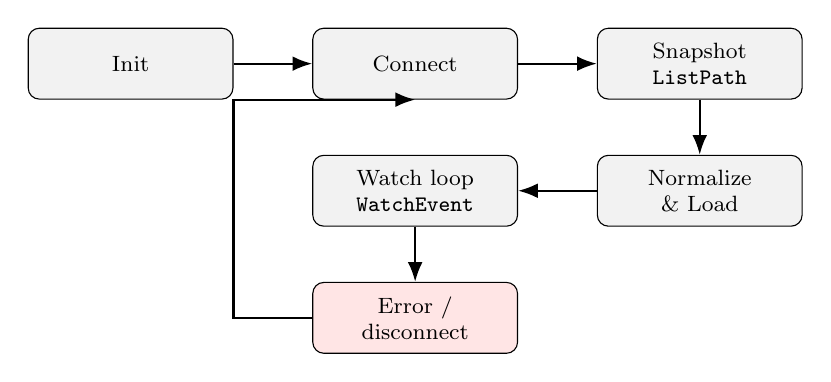
\begin{tikzpicture}[node distance=0.7cm and 1.0cm,every node/.style={font=\footnotesize}]
\node[state, fill=gray!10] (init)    {Init};
\node[state, fill=gray!10, right=of init]   (conn)    {Connect};
\node[state, fill=gray!10, right=of conn]   (snap)    {Snapshot\\\texttt{ListPath}};
\node[state, fill=gray!10, below=of snap]   (load)    {Normalize\\\& Load};
\node[state, fill=gray!10, left=of load]    (watch)   {Watch loop\\\texttt{WatchEvent}};
\node[state, fill=red!10, below=of watch]   (err)     {Error /\\disconnect};

\draw[msarr] (init) -- (conn);
\draw[msarr] (conn) -- (snap);
\draw[msarr] (snap) -- (load);
\draw[msarr] (load) -- (watch);
\draw[msarr] (watch) -- (err);
\draw[msarr] (err.west) -- ++(-1,0) |- (conn.south);
\end{tikzpicture}
\caption{Конечный автомат жизненного цикла повторного подключения и ресинхронизации}
\label{fig:lifecycle}
\end{figure}

\subsection{Модель состояния и корректность}

Снимок и поток удобно рассматривать не как противоположности, а как две
фазы жизни одного и того же материализованного состояния. Снимок нужен
при старте, при пересинхронизации и при выгрузке полной таблицы наружу.
Поток снижает задержку актуализации состояния, применяет
инкрементальные изменения отдельных префиксных записей и передаёт
обновления подписчикам.

Порядок применения событий задаётся самой сессией с GoBGP: сервис
обрабатывает их в том порядке, в котором они приходят. По терминологии
работ по обработке потоков~\cite{akidau2015dataflow} это
\textit{processing-time}, а не \textit{event-time}. Для прикладной
задачи такой выбор обоснован по двум причинам. Во-первых, истинное время
события у исходного BGP-роутера сервису недоступно -- между ним и
сервисом стоит GoBGP, агрегирующий поток. Во-вторых, важна не глобальная
синхронизация по астрономическим часам, а локальная согласованность
шагов: после применения события $e_i$ и до применения $e_{i+1}$ ответы
на \texttt{Lookup} должны соответствовать состоянию после $e_i$. Эта
гарантия обеспечивается дисциплиной работы с \texttt{prefixStore}:
события обрабатываются по одному, а видимость их результата управляется
блокировками внутри шардов.

Кратко состояние таблицы записывается как
\[
S_n = f(S_0, e_1, e_2, \ldots, e_n),
\]
где $S_0$ -- результат начальной загрузки, а $e_1, \ldots, e_n$ --
последовательно применённые BGP-события. Любой ответ \texttt{Lookup}
клиента $C$ в момент $t_C$ соответствует состоянию после некоторого числа
применённых событий $S_k$, $k \le n(t_C)$. Полная выгрузка
\texttt{GetPrefixesASTable} возвращает текущее представление состояния
сервиса; в шардированной реализации её согласованность уточняется в
главе~\ref{sec:art-storage}. Подписка \texttt{SubscribePrefixASUpdates}
даёт поток дельт, который позволяет клиенту, начав с $S_k$, восстановить
$S_{k+1}, S_{k+2}, \ldots$ Из этой записи видно главное: снимок и поток
связаны единой семантикой, а \texttt{Replace} после ресинхронизации --
переустановка базовой точки $S_0$ при сохранении того же типа функции
$f$.

%==============================================================

\section{Реализация шардированного ART-хранилища}

\subsection{Общая идея шардирования}

Одно из ограничений любой общей in-memory структуры заключается в
конкуренции за блокировки. Если все операции чтения и записи проходят
через одно дерево и один lock, то потоковая модель быстро упрётся в
contention. Поэтому в работе применяется шардирование.

Ключ префикса хешируется (используется FNV-32a), и значение хеша по
модулю числа шардов определяет, в какой шард он попадёт. Каждый шард
содержит собственное ART-дерево и собственный
\texttt{sync.RWMutex}. Такой подход даёт два преимущества:

\begin{itemize}
\item обновления разных префиксов, попадающих в разные шарды, не
конкурируют напрямую;
\item чтение и запись локализуются внутри одного шарда.
\end{itemize}

Устройство шардированного хранилища изображено на
рис.~\ref{fig:shards}.

\begin{figure}[ht]
\centering
\begin{tikzpicture}[node distance=0.4cm and 0.4cm,every node/.style={font=\footnotesize}]
\node[block, text width=3.0cm] (fv)  {Полный снимок\\ или update-событие};
\node[block, text width=4.0cm, below=of fv] (h)  {FNV-32a хеш\\ и маршрутизация по шардам};

\node[block2, below=1.0cm of h, xshift=-3.6cm] (lo0) {Загрузчик 0};
\node[block2, below=1.0cm of h, xshift=-1.2cm] (lo1) {Загрузчик 1};
\node[font=\large, below=1.0cm of h, xshift=0.5cm] {$\cdots$};
\node[block2, below=1.0cm of h, xshift=2.6cm] (lok) {Загрузчик $K{-}1$};

\node[block2, fill=gray!18, below=0.4cm of lo0] (a0) {ART$_0$};
\node[block2, fill=gray!18, below=0.4cm of lo1] (a1) {ART$_1$};
\node[font=\large, below=0.4cm of h, xshift=0.5cm, yshift=-1.0cm] {};
\node[block2, fill=gray!18, below=0.4cm of lok] (ak) {ART$_{K-1}$};

\draw[msarr] (fv) -- (h);
\draw[msarr] (h.south) -- (lo0.north);
\draw[msarr] (h.south) -- (lo1.north);
\draw[msarr] (h.south) -- (lok.north);
\draw[msarr] (lo0) -- (a0);
\draw[msarr] (lo1) -- (a1);
\draw[msarr] (lok) -- (ak);
\end{tikzpicture}
\caption{Устройство шардированного ART-хранилища}
\label{fig:shards}
\end{figure}

\subsection{Внутреннее представление ключа}

Для хранения в ART IP-префикс переводится в байтовое представление,
удобное для лексикографической навигации по дереву. Этот этап важен,
потому что ART работает на последовательности байтов, а не на
абстрактном объекте «префикс». Соответственно, корректное кодирование
ключа определяет корректность дальнейших операций поиска и обхода
\cite{leis2013art}. В реализации используется фиксированная длина
кодирования с явной длиной маски, что упрощает дальнейший longest
prefix match.

\subsection{Lookup по IP-адресу}

Точечный lookup для внешнего клиента реализует longest prefix match по
текущему состоянию хранилища. В зависимости от способа организации
ключей и навигации по дереву возможны разные стратегии:

\begin{itemize}
\item хранение всех префиксов и поиск наиболее специфичного кандидата;
\item последовательная проверка длин масок (до~33 для IPv4 и до~129
для IPv6);
\item более сложная навигация по radix-структуре с удержанием
последнего совпадения вдоль пути.
\end{itemize}

В текущей реализации lookup имеет приемлемые характеристики для IPv4
и более высокую стоимость для IPv6, что связано с особенностями
перебора масок и большей глубиной адресного пространства. Возможные
направления оптимизации обсуждаются в главе~10.

\subsection{Upsert и delete}

Главное достоинство нового backend-хранилища проявляется именно на
операциях обновления. \texttt{Upsert} затрагивает один шард и локально
модифицирует его дерево; \texttt{Delete} обрабатывает withdraw-событие
точно так же~-- локально, без перестройки остальных шардов. Это
принципиально отличается от поведения batch-структуры, в которой
каждое изменение маршрута приводило к полной перестройке таблицы.

\subsection{Dump полного состояния}

Полная выгрузка в ART-режиме реализуется как обход всех шардов и
сборка результатов. Это естественно делает \texttt{Dump} дороже, чем в
структуре, которая держит уже готовый линейный массив записей. По
сути, ART-подход платит за mutability дополнительной ценой обхода,
аллокаций и (опционально) последующей сортировки. В реализации
сортировка управляется параметром \texttt{ASMAP\_STORE\_ART\_DUMP\_SORT},
что позволяет в сценариях, где порядок не важен, экономить заметную
долю времени на больших таблицах.

Эта особенность не является дефектом реализации как таковым. Она
отражает фундаментальный компромисс: структура, оптимизированная под
частые инкрементальные обновления, редко оказывается одновременно
лучшей и для операции «отдать всё содержимое сразу».

\subsection{Контракт \texttt{prefixStore}}

С точки зрения исследовательской работы важна не сама конкретная
реализация, а наличие явного контракта \texttt{prefixStore}, общего
для двух backend-вариантов. Контракт задан минимальным набором
операций, описанных в табл.~\ref{tab:store-contract}; это делает
сравнение реализаций честным и сводит экспериментальный анализ к
сопоставлению поведения двух конкретных воплощений одного и того же
интерфейса.

\begin{table}[ht]
\centering
\caption{Контракт \texttt{prefixStore} и принципиальное поведение реализаций}
\label{tab:store-contract}
\small
\begin{tabular}{>{\raggedright\arraybackslash}p{2.6cm}>{\raggedright\arraybackslash}p{4.6cm}>{\raggedright\arraybackslash}p{5.6cm}}
\toprule
Операция & Реализация \textit{ranger} & Реализация \textit{шард. ART} \\
\midrule
\texttt{Replace} & полная замена слайса
                 & параллельная загрузка по шардам \\
\texttt{Upsert}  & пересборка всего слайса и полная замена ($O(n)$)
                 & локальная модификация одного шарда ($O(\log n / K)$ амортизированно) \\
\texttt{Delete}  & пересборка всего слайса
                 & локальное удаление в одном шарде \\
\texttt{Lookup}  & longest prefix match по линейной структуре
                 & longest prefix match по ART-дереву соответствующего шарда \\
\texttt{Dump}    & копирование готового слайса (1~аллокация)
                 & обход всех $K$ шардов, опционально сортировка \\
\bottomrule
\end{tabular}
\end{table}

\subsection{Целевая операция и интерпретация результатов}

Оценивать новое хранилище по одному только времени \texttt{Dump} или
по latency точечного \texttt{Lookup} некорректно. Целевая функция
работы другая -- сделать потоковую актуализацию реализуемой на
практике. Главной метрикой здесь становится стоимость
\texttt{Upsert} и \texttt{Delete}, а \texttt{Dump} и \texttt{Lookup}
играют роль «расходов на остальные сценарии». Эту установку важно
удерживать при чтении главы~9, где приведены эмпирические результаты.

\subsection{Согласованность параллельного доступа}

Шардирование само по себе не определяет модель согласованности; оно
лишь снижает контеншн между независимыми операциями. Чтобы
\texttt{Lookup} и \texttt{Upsert} безопасно сосуществовали внутри
одного шарда, в реализации используется стандартный
read-write-mutex. Все операции записи (\texttt{Upsert},
\texttt{Delete}, локальная фаза \texttt{Replace}) удерживают
write-lock соответствующего шарда; \texttt{Lookup} удерживает
read-lock того шарда, в котором происходит поиск.

Такая дисциплина даёт следующие гарантии:

\begin{itemize}
\item внутри одного шарда параллельные \texttt{Lookup}
выполняются без взаимного блокирования;
\item модификация одного шарда не блокирует операции в других
шардах;
\item \texttt{Dump} не требует глобального write-lock и реализуется
последовательным захватом read-lock каждого шарда либо
параллельным обходом независимых шардов с локальными read-lock.
\end{itemize}

Важно отметить, что согласованность \texttt{Dump} в этой модели
является \textit{шардовой}, а не глобальной snapshot-согласованностью
во всём дереве: каждое значение, появившееся в дампе, корректно
относительно своего шарда в момент чтения. Для прикладного сценария
получения полной таблицы это допустимо, поскольку клиент
интерпретирует результат как «текущее представление сервиса»,
а не как атомарный одномоментный срез всех шардов.

При необходимости более сильной семантики можно либо ввести
дополнительный механизм глобального snapshot (например, версионирование
шардов), либо ограничиться тем, что глобальный «строгий» snapshot
по построению не нужен в логике downstream-клиентов: они и так
строят своё состояние как $S_0 + \Delta$ через подписку.

\subsection{Поведение во время ресинхронизации}

Отдельный важный режим работы -- ресинхронизация. В этот момент
сервис должен:

\begin{enumerate}
\item получить новый снимок;
\item подготовить из него корректное внутреннее представление;
\item заменить текущее состояние store на новое;
\item возобновить обработку потока обновлений.
\end{enumerate}

В шардированной реализации эта последовательность выполняется как
скоординированная замена содержимого всех шардов; параллельный
\texttt{Lookup}, попадающий в момент перестроения, либо обслуживается
из частично уже обновлённого состояния, либо ожидает завершения
write-фазы конкретного шарда. Аномалии «исчезновения» ранее
существовавшего префикса в этот момент возможны, но они являются
ожидаемым следствием ресинхронизации и кратковременны. Учитывая, что
ресинхронизация происходит редко (только при сбоях или после
длительных пауз), такая модель является разумным инженерным
компромиссом.

%==============================================================

\section{Методика и организация экспериментов}
\label{sec:methodology}

\subsection{Цель экспериментальной части}

Экспериментальная часть должна ответить на вопрос, подтверждается ли
выдвинутая гипотеза -- в части возможности потокового обновления
in-memory базы после выделения микросервиса. Для этого нужно измерить,
как новое и прежнее внутренние хранилища ведут себя на наборе операций, соответствующих
реальным сценариям использования сервиса:

\begin{itemize}
\item полная выгрузка таблицы (\texttt{Dump});
\item одиночное обновление маршрута (\texttt{Upsert});
\item точечный поиск по IP-адресу (\texttt{Lookup});
\item влияние числа шардов на ключевые операции;
\item различия между IPv4 и IPv6.
\end{itemize}

\subsection{Сравниваемые варианты}

В опытах сравниваются:

\begin{itemize}
\item \textbf{\texttt{ranger}} -- прежний вариант хранилища на базе
библиотеки \texttt{ranger};
\item \textbf{шард. ART} -- новый вариант хранилища на базе шардированного
Adaptive Radix Tree.
\end{itemize}

Это важный методический момент: сравнение выполняется не между двумя
абстрактными структурами данных из учебника, а между двумя реальными
вариантами внутреннего хранилища одного и того же сервиса с одним и тем же
\texttt{prefixStore}-контрактом. Все различия, фиксируемые в
эксперименте, можно интерпретировать как различия между
реализацией, ориентированной на полную замену, и реализацией,
ориентированной на поток обновлений, в рамках этого
контракта.

\subsection{Конфигурация стенда}

Параметры экспериментального стенда приведены в
табл.~\ref{tab:bench-setup}. Все измерения проводились на одной и той
же физической машине, без использования контейнеров и виртуализации,
с зафиксированным набором фоновых процессов.

\begin{table}[ht]
\centering
\caption{Конфигурация стенда экспериментов}
\label{tab:bench-setup}
\small
\begin{tabular}{>{\raggedright\arraybackslash}p{4.5cm}>{\raggedright\arraybackslash}p{8.5cm}}
\toprule
Параметр & Значение \\
\midrule
CPU                  & AMD Ryzen AI 9 HX 370 (24 потока) \\
ОЗУ                  & 32 ГБ LPDDR5X \\
Среда                & Linux x86\_64 \\
Среда исполнения     & Go 1.24+ \\
Инструмент           & \texttt{go test -bench} с теговой подсистемой \texttt{bench}, \texttt{benchheavy} \\
ART-параметры        & 16 шардов, \texttt{WithDumpSort(false)} в сценариях с большими $n$ \\
	Размеры таблиц       & $n \in \{1\,000;\, 10\,000;\, 100\,000\}$; отдельный тяжёлый сценарий -- $3\,000\,000$ смешанных IPv4/IPv6 записей \\
	Семейства адресов    & IPv4 \texttt{/24} (искусственные диапазоны \texttt{10.x.y.0/24}, \texttt{11.x.y.0/24}), IPv6 \texttt{/64} в \texttt{2001:db8::/32}; для тяжёлого сценария -- смесь IPv4 \texttt{/24} и IPv6 \texttt{/64} \\
Параметры запуска    & \texttt{count=2}, \texttt{benchtime=400ms}\,/\,\texttt{500ms} \\
\bottomrule
\end{tabular}
\end{table}

\subsection{Наборы данных и сценарии}

Для измерений используются синтетические наборы префиксов, а также
сценарии, имитирующие реалистичную нагрузку. В частности:

\begin{itemize}
\item таблицы различного размера, вплоть до~$10^5$ префиксов в основных
сериях и отдельный тяжёлый сценарий на $3\cdot10^6$ смешанных записей;
\item отдельные наборы для IPv4 и IPv6;
\item сценарии полного \texttt{Dump};
\item сценарии одиночного \texttt{Upsert} поверх уже загруженной
таблицы;
\item сценарии \texttt{Lookup};
\item sweep по числу шардов $K \in \{1,8,16,32,64\}$.
\end{itemize}

Такой дизайн эксперимента позволяет отдельно оценить операции, которые
ограничивают применимость каждой реализации: полную выгрузку, точечный
поиск, инкрементальное обновление и влияние числа шардов.

\subsection{Почему именно эти метрики достаточны}

Для данной работы важно подчеркнуть, что метрики выбираются не
случайно, а отражают конкретные эксплуатационные сценарии.

Операция \texttt{Dump} соответствует сценарию получения полного снимка
внешним потребителем, а также внутренним этапам начальной инициализации и
ресинхронизации.

Операция \texttt{Upsert} соответствует основной сущности потокового
режима: локальному отражению одного BGP-изменения. Именно её стоимость
определяет, осмыслен ли переход от полной пересборки таблицы к потоку;
измерение \texttt{Upsert} -- прямая проверка этой части гипотезы, а не
«бенчмарк ради ART».

Операция \texttt{Lookup} задаёт дополнительный разрез: приемлемость
задержки точечного запроса при выбранном хранилище (включая реализацию
LPM).

Измерение при разных значениях числа шардов показывает, где проходит
граница между полезной параллельностью и издержками чрезмерного дробления
состояния.

Именно эта совокупность метрик позволяет проверить, достигнута ли
цель перехода к потоковой архитектуре, и подтвердить или
опровергнуть выдвинутую гипотезу.

\subsection{Ограничения экспериментальной методики}

Экспериментальная часть измеряет прежде всего внутренние операции
хранилища: полную загрузку, точечный поиск, инкрементальное обновление и
полную выгрузку таблицы. Такой выбор позволяет изолировать различия между
двумя реализациями \texttt{prefixStore}, но оставляет за пределами
измерений ряд факторов эксплуатации:

\begin{itemize}
\item сетевые задержки в внешних gRPC-вызовах;
\item долгосрочную динамику при реальном потоке BGP update-событий за
большие интервалы времени;
\item поведение под многоклиентской нагрузкой на пользовательский API;
\item влияние сборщика мусора и давления на аллокатор при длительной
работе сервиса;
\item воспроизведение реалистичного распределения длин префиксов из
промышленных BGP-таблиц.
\end{itemize}

Для цели данной работы такое ограничение методики приемлемо: измерения
проверяют именно тот слой, в котором различаются \texttt{ranger} и
шардированный ART, и позволяют сравнить два варианта хранилища по
ключевым операциям.
Ограничения интерпретации результатов перечислены выше и учитываются в
выводах главы~\ref{sec:experiment-results}.

%==============================================================

\section{Результаты экспериментов и их интерпретация}
\label{sec:experiment-results}

\subsection{Полная выгрузка}

Измерения показывают, что вариант хранилища, основанный на
\texttt{ranger}, быстрее выполняет полную выгрузку таблицы. Это объясняется
тем, что он концептуально хранит уже подготовленный линейный набор
записей и может отдавать его почти как копию готового массива.
Шардированный ART, напротив, должен обойти все шарды, декодировать
ключи, собрать raw-префиксы и построить непересекающуюся таблицу для
внешней выдачи.

Конкретные численные результаты для $n=100000$ приведены в
табл.~\ref{tab:bench-dump}. Во всех ART-сценариях сортировка дампа
отключена; измерение включает построение непересекающейся таблицы.

\begin{table}[ht]
\centering
\caption{Бенчмарк \texttt{Dump} для $n=100000$}
\label{tab:bench-dump}
\footnotesize
\begin{tabular}{>{\raggedright\arraybackslash}p{4.2cm}rr}
\toprule
Сценарий & \texttt{ranger} & ART \\
\midrule
IPv4 \texttt{Dump} & $48{,}90$ мс/оп. & $142{,}80$ мс/оп. \\
IPv6 \texttt{Dump} & $101{,}36$ мс/оп. & $201{,}93$ мс/оп. \\
\bottomrule
\end{tabular}
\end{table}

Эти данные фиксируют проигрыш ART по полной выгрузке. Для целевого профиля
нагрузки это не опровергает гипотезу, поскольку \texttt{Dump} не является
основным рабочим режимом потоковой модели, но задаёт ограничение для
сценариев частых полных выгрузок.

\subsection{Инкрементальное обновление}

С точки зрения постановки задачи этот раздел -- центральный: он
показывает, что потоковое применение одиночных BGP-изменений к
in-memory базе технически осуществимо, а не только объявлено в
архитектуре. Именно на операции одиночного \texttt{Upsert} ART-подход
демонстрирует решающее преимущество (табл.~\ref{tab:bench-upsert}).
Обе реализации поддерживают точечное изменение состояния, но ART
выполняет эту операцию локально в одном шарде и требует меньше времени и
аллокаций.

\begin{table}[ht]
\centering
\caption{Бенчмарк одиночного \texttt{Upsert} поверх заполненной
таблицы, $n=100000$}
\label{tab:bench-upsert}
\small
\begin{tabular}{lrr}
\toprule
Сценарий & \texttt{ranger} & ART \\
\midrule
IPv4 \texttt{Upsert} & $3{,}94$ мкс/оп. & $173{,}1$ нс/оп. \\
IPv6 \texttt{Upsert} & $6{,}43$ мкс/оп. & $199{,}2$ нс/оп. \\
\bottomrule
\end{tabular}
\end{table}

Разница составляет десятки раз при $n=10^5$. Это главный эмпирический
аргумент в пользу ART для потоковой модели: отдельное BGP-событие
применяется с малой задержкой и небольшим числом аллокаций, а значит
инкремент становится естественным базовым режимом внутри выделенного
микросервиса с общим API.

\subsection{Lookup по IP}

Это вспомогательный разрез относительно центральной цели работы
(микросервис и поток обновлений), но он фиксирует цену точечного чтения
после выбора структуры. По операции \texttt{Lookup} обе реализации дают
сопоставимую задержку. ART проверяет только активные длины префиксов,
поэтому стоимость поиска не определяется полным диапазоном возможных
масок IPv4 или IPv6. Результаты приведены в табл.~\ref{tab:bench-lookup}.

\begin{table}[ht]
\centering
\caption{Бенчмарк \texttt{Lookup}, $n \approx 10^5$}
\label{tab:bench-lookup}
\small
\begin{tabular}{lrr}
\toprule
Сценарий       & \texttt{ranger}       & ART (16 шардов) \\
\midrule
IPv4 & $\approx 150$--$180\,$нс/оп. & $\approx 150\,$нс/оп. \\
IPv6 & $175{,}5\,$нс/оп. & $211{,}7\,$нс/оп. \\
\bottomrule
\end{tabular}
\end{table}

Эти данные показывают, что \texttt{Lookup} остаётся пригодным для
синхронного gRPC-запроса. ART не является универсальным победителем по
всем метрикам, но после учёта активных длин префиксов разрыв по чтению
практически устранён.

\subsection{Влияние числа шардов}

Эксперименты показывают, что увеличение числа шардов не даёт линейного
ускорения всех операций. Для последовательного \texttt{Lookup} выигрыш
находится в пределах шума. Для \texttt{Dump} большое число шардов
ухудшает результат из-за роста служебных издержек и последующего
глобального flatten (табл.~\ref{tab:bench-shards}). Для конкурентных
update-сценариев шардирование остаётся полезным, потому что снижает
конкуренцию между независимыми модификациями.

\begin{table}[ht]
\centering
\caption{Измерение ART при разном числе шардов на смешанном наборе
$3\cdot10^6$ записей}
\label{tab:bench-shards}
\small
\begin{tabular}{lrr}
\toprule
$K$ (шардов) & \texttt{Lookup} & \texttt{Dump} \\
\midrule
$1$  & $175{,}1$ нс/оп. & $3{,}62$ с/оп. \\
$8$  & $176{,}4$ нс/оп. & $4{,}99$ с/оп. \\
$16$ & $175{,}9$ нс/оп. & $5{,}59$ с/оп. \\
$32$ & $175{,}6$ нс/оп. & $6{,}24$ с/оп. \\
$64$ & $177{,}8$ нс/оп. & $6{,}89$ с/оп. \\
\bottomrule
\end{tabular}
\end{table}

Следовательно, число шардов является параметром настройки, а не
правилом «чем больше, тем лучше». Для dump-heavy сценариев лучший
результат показывает один шард; для конкурентных read/write-нагрузок
практически разумной остаётся зона умеренного шардирования.

\subsection{Поведение IPv6}

IPv6 заслуживает отдельного внимания. По \texttt{Dump} ART остаётся
медленнее \texttt{ranger}, поскольку полная выдача включает построение
непересекающейся таблицы. По \texttt{Upsert} ART сохраняет преимущество:
$199{,}2$ нс/оп. против $6{,}43$ мкс/оп. у \texttt{ranger}. По
\texttt{Lookup} результат сопоставим: $211{,}7$ нс/оп. у ART против
$175{,}5$ нс/оп. у \texttt{ranger}.

\subsection{Смешанный набор на 3 млн записей}

Для проверки масштабирования был отдельно выполнен тяжёлый прогон на
$3\,000\,000$ префиксных записей в смешанном режиме: IPv4 \texttt{/24} и
IPv6 \texttt{/64}. ART использовался с 16 шардами и выключенной
сортировкой полной выгрузки. Результаты приведены в
табл.~\ref{tab:bench-3m-mixed}.

\begin{table}[ht]
\centering
\caption{Сравнение \texttt{ranger} и шардированного ART на смешанном наборе из $3\cdot10^6$ записей}
\label{tab:bench-3m-mixed}
\small
\resizebox{\textwidth}{!}{%
\begin{tabular}{lrrr}
\toprule
Сценарий & \texttt{ranger} & ART (16 шардов, без сортировки) & Победитель \\
\midrule
\texttt{Replace} / полная загрузка
  & $30{,}84$ с/оп.
  & $693{,}98$ мс/оп.
  & ART \\
\texttt{Lookup}
  & $187{,}8$ нс/оп.
  & $176{,}7$ нс/оп.
  & ART \\
\texttt{Dump}
  & $4{,}25$ с/оп.
  & $6{,}16$ с/оп.
  & \texttt{ranger} \\
\texttt{Upsert}
  & $7{,}99$ мкс/оп.
  & $255{,}5$ нс/оп.
  & ART \\
\bottomrule
\end{tabular}
}
\end{table}

Та же серия измерений показывает высокую стоимость полной выгрузки по
памяти. Для \texttt{Dump} на $3\cdot10^6$ записей без искусственного
memory pressure \texttt{ranger} выделяет около $10{,}88$~GiB/оп.,
ART с одним шардом -- около $11{,}41$~GiB/оп., ART с 32 шардами --
около $11{,}82$~GiB/оп. При \texttt{GOMEMLIMIT=1GiB} операция
завершается, но заметно замедляется из-за GC: \texttt{ranger} занимает
около $11{,}09$~с, ART с одним шардом -- около $13{,}71$~с, ART с
8 шардами -- около $11{,}26$~с. Для ART при \texttt{GOMEMLIMIT=2GiB}
штраф в этом бенчмарке почти исчезает.

Этот прогон уточняет общую картину. На большой смешанной таблице ART
выигрывает в полной загрузке состояния, точечном поиске и
инкрементальном обновлении. Основная дорогая операция для ART --
полный \texttt{Dump} с построением непересекающейся таблицы.
Следовательно, выбор хранилища зависит от профиля нагрузки: для
состояния, обновляемого потоком BGP-событий, критичны \texttt{Replace}
и \texttt{Upsert}, тогда как для сценариев частой полной выгрузки нужен
кэшированный или потоковый вариант \texttt{Dump}.

\subsection{Сводный итог сравнения}

Сводка по сценариям приведена в табл.~\ref{tab:bench-summary}.

\begin{table}[ht]
\centering
\caption{Итоговая сводка: какой вариант хранилища выигрывает в каком сценарии}
\label{tab:bench-summary}
\small
\begin{tabular}{>{\raggedright\arraybackslash}p{4.0cm}lp{6.5cm}}
\toprule
Сценарий & Победитель & Комментарий \\
\midrule
Полная выгрузка
  & \texttt{ranger}
  & ART выполняет обход дерева и строит непересекающуюся таблицу \\
Одиночный \texttt{Upsert}
  & ART
  & десятки раз преимущества; решающий фактор для потокового режима \\
\texttt{Lookup} IPv4
  & сопоставимо
  & фильтрация по активным длинам префикса даёт близкую задержку у обеих реализаций \\
\texttt{Lookup} IPv6
  & сопоставимо
  & \texttt{ranger} быстрее примерно в 1{,}2 раза на $n=10^5$ \\
Полная загрузка \texttt{Replace} на $3\cdot10^6$ записей
  & ART
  & $693{,}98$ мс/оп. против $30{,}84$ с/оп. у \texttt{ranger} \\
Потоковое обновление
  & ART
  & отдельное BGP-событие применяется с малой задержкой и небольшим числом аллокаций \\
Потоковое обновление на $3\cdot10^6$ записей
  & ART
  & \texttt{Upsert}: $255{,}5$ нс/оп. против $7{,}99$ мкс/оп. у \texttt{ranger} \\
\bottomrule
\end{tabular}
\end{table}

Из сводки следуют четыре вывода, непосредственно связанные с измеренными
операциями:

\begin{enumerate}
\item \texttt{ranger} сохраняет преимущество в сценариях частой полной
выгрузки: на смешанном наборе $3\cdot10^6$ записей \texttt{Dump} у
\texttt{ranger} занимает $4{,}25$ с/оп. против $6{,}16$ с/оп. у ART;
\item ART лучше соответствует сценарию потокового применения BGP-событий:
одиночный \texttt{Upsert} на смешанном наборе выполняется за
$255{,}5$ нс/оп., тогда как для \texttt{ranger} та же операция занимает
$7{,}99$ мкс/оп.;
\item на полной загрузке большого смешанного набора ART также показывает
меньшее время: \texttt{Replace} занимает $693{,}98$ мс/оп. против
$30{,}84$ с/оп. у \texttt{ranger};
\item практический выбор реализации зависит от профиля нагрузки: для
сервиса, который должен регулярно применять инкрементальные BGP-обновления
и быстро выполнять полную загрузку состояния, измерения подтверждают
преимущество ART; для частых полных выгрузок нужен кэшированный или
потоковый \texttt{Dump}.
\end{enumerate}

Последний вывод задаёт границу применимости результата. Выделение функции
в микросервис и единый gRPC контракт для нескольких продуктов образуют
самостоятельный архитектурный слой; шардированный ART снижает время
потокового обновления по сравнению с \texttt{ranger}-backend-ом.

\subsection{Совокупная стоимость потокового профиля нагрузки}

Чтобы перевести бенчмарки в эксплуатационно содержательную плоскость для
уже выделенного микросервиса, полезно построить простую модель
совокупной стоимости. Для поддержания актуальной таблицы
\texttt{prefix -> ASN} ключевым режимом является не полная выгрузка
состояния, а регулярное применение инкрементальных BGP-обновлений.
Поэтому проигрыш ART в операции \texttt{Dump} сам по себе не определяет
выбор хранилища: его нужно сопоставлять со стоимостью \texttt{Upsert},
\texttt{Delete} и \texttt{Lookup} в установившемся потоковом профиле
нагрузки. Рассмотрим режим, в котором:

\begin{itemize}
\item в системе хранится таблица из $n$ префиксов
($n \in \{10^4;\,10^5\}$);
\item за единицу времени происходит $\lambda$ инкрементальных
обновлений (Upsert/Delete);
\item клиенты выполняют $\mu$ запросов \texttt{Lookup} в секунду;
\item операция полного \texttt{Dump} вызывается с частотой $\nu$ в
секунду.
\end{itemize}

Тогда суммарную CPU-нагрузку на хранилище можно оценить как

\[
C(\lambda,\mu,\nu) =
   \lambda \cdot t_{\mathrm{upsert}}(n)
 + \mu    \cdot t_{\mathrm{lookup}}(n)
 + \nu    \cdot t_{\mathrm{dump}}(n),
\]

где $t_{\mathrm{upsert}}$, $t_{\mathrm{lookup}}$ и
$t_{\mathrm{dump}}$ -- это средние времена соответствующих операций,
взятые из табл.~\ref{tab:bench-dump}--\ref{tab:bench-shards}.

Подставим типичные значения для $n = 10^5$:

\begin{itemize}
\item \texttt{ranger}: $t_{\mathrm{upsert}} \approx 3{,}94 \cdot 10^{-6}$ с;
$t_{\mathrm{lookup}} \approx 1{,}5 \cdot 10^{-7}$ с;
$t_{\mathrm{dump}} \approx 4{,}89 \cdot 10^{-2}$ с;
\item шард. ART: $t_{\mathrm{upsert}} \approx 1{,}7 \cdot 10^{-7}$ с;
$t_{\mathrm{lookup}} \approx 1{,}5 \cdot 10^{-7}$ с;
$t_{\mathrm{dump}} \approx 1{,}43 \cdot 10^{-1}$ с.
\end{itemize}

Сравнение совокупной стоимости для двух представительных профилей
нагрузки приведено в табл.~\ref{tab:bench-cost}.

\begin{table}[ht]
\centering
\caption{Оценка совокупной CPU-стоимости в установившемся режиме при
$n = 10^5$ (приближённо, CPU-с/с $=$ доля одного CPU-ядра на каждую
секунду физического времени)}
\label{tab:bench-cost}
\small
\begin{tabular}{lrr}
\toprule
Сценарий & \texttt{ranger} & шард. ART \\
\midrule
$\lambda{=}10$, $\mu{=}10^4$, $\nu{=}10^{-2}$
	   & $\approx 0{,}0020$ CPU-с/с
	   & $\approx 0{,}0029$ CPU-с/с \\
$\lambda{=}10^3$, $\mu{=}10^5$, $\nu{=}10^{-2}$
	   & $\approx 0{,}019$ CPU-с/с
	   & $\approx 0{,}017$ CPU-с/с \\
\bottomrule
\end{tabular}
\end{table}

Числа в табл.~\ref{tab:bench-cost} имеют ясную интерпретацию. Оба
варианта остаются на уровне малой доли одного ядра для рассмотренных
профилей, но структура затрат различается: у ART дешевле обновления, а
у \texttt{ranger} дешевле полный \texttt{Dump}. Поэтому профиль нагрузки
определяет выбор backend-а и необходимость кэширования полной выгрузки.

Более того, в этой модели хорошо видно, что доминирующая статья расходов
меняется в зависимости от режима. При частых изменениях важна стоимость
\texttt{Upsert}/\texttt{Delete}; при частых полных выгрузках начинает
доминировать \texttt{Dump} и построение flattened-представления.

Если переложить те же цифры в плоскость требований к задержке
актуализации, важным становится время применения отдельного события.
Пусть допустимая задержка актуализации таблицы
$T_{\mathrm{stale}} \le 1$~с. Потоковая модель достигает этого за счёт
обработки отдельных событий: каждое обновление применяется за единицы
микросекунд или быстрее, а полная выгрузка остаётся отдельным
ресурсно-ёмким сценарием.

%==============================================================

\section{Практические ограничения и направления развития}
\label{sec:limitations}

\subsection{Ограничения текущей реализации}

Несмотря на положительные результаты по линии «микросервис + потоковое
обновление», текущая реализация имеет ряд ограничений.

Во-первых, \texttt{Dump} остаётся дороже, чем у \texttt{ranger}. В прикладном
сценарии это допустимо, если полный снимок вызывается сравнительно
редко, но при интенсивном использовании полного дампа может
понадобиться дополнительный кэшированный слой полного снимка или
потоковая выдача результата. Основная стоимость связана с построением
непересекающейся таблицы для внешних потребителей.

Во-вторых, полный \texttt{Dump} на миллионах записей создаёт большой
поток аллокаций. При жёстком \texttt{GOMEMLIMIT} операция завершается,
но замедляется из-за работы GC, поэтому production-конфигурация должна
учитывать параллельную нагрузку, gRPC buffers и возможную ресинхронизацию.

В-третьих, потоковая модель пока в основном рассматривается как
последовательность update-событий из одного источника. Для более
сложных промышленных сценариев могут понадобиться расширенные гарантии
повторной доставки, дедупликации и диагностики пропущенных событий
\cite{kreps2011kafka,kleppmann2017ddia}.

\subsection{Возможные доработки реализации}

Ограничения, выявленные в экспериментальной части, указывают на три
группы доработок текущей реализации.

\textit{Lookup.} Операция LPM поверх ART использует наборы активных длин
префикса и поэтому проверяет только релевантные кандидатные маски.
Дальнейшая доработка может состоять в хранении признака терминальности
непосредственно в узлах дерева, сохранении последнего найденного
валидного совпадения во время прохода по ключу и разделении быстрых путей
обработки для IPv4 и IPv6. Работы
Tree~Bitmap~\cite{eatherton2004treebitmap} и
Poptrie~\cite{asai2015poptrie} показывают близкие приёмы оптимизации
поиска наиболее специфичного префикса.

\textit{Dump.} Для редких, но дорогих полных выгрузок логично ввести
кэшированный упорядоченный снимок, ленивую материализацию или
потоковую выдачу содержимого вместо одного большого ответа. Если
сервис начнёт использоваться как поставщик периодических выгрузок,
полезны и дифференциальные снимки для конкретных подписчиков.

\textit{Телеметрия.} Расширение телеметрии и интеграция с
BMP-наблюдением~\cite{rfc7854} и публичными
коллекторами~\cite{ripe-ris,routeviews} позволят измерять задержку
актуализации, число принятых и пропущенных update-событий, время
ресинхронизации, размеры очередей и ошибки соединения с GoBGP. Сравнение
локальной таблицы с независимым внешним источником также может служить
сигналом потери или неправильной интерпретации событий. Здесь же уместен
механизм, аналогичный route flap damping~\cite{rfc2439}, для подавления
гиперактивных префиксов.

Шаблон «отдельный сервис с единым API + снимок + поток + шардированное
in-memory ядро» переносим за пределы рассмотренной пары продуктов. Он
применим в системах сетевой безопасности, аналитике трафика,
операторской отчётности и сетевом инвентаре -- везде, где нужно держать
актуальный маршрутный контекст для принятия решений и не дублировать
логику между потребителями.

%==============================================================

\section*{ЗАКЛЮЧЕНИЕ}

Работа посвящена поддержанию актуального соответствия
\textit{IP-префикс~$\rightarrow$~ASN} по данным BGP для продуктов BIFIT
MITIGATOR и BIFIT COLLECTOR. Главный результат -- переход от
периодической полной перестройки таблицы к потоковому обновлению
in-memory состояния в отдельном микросервисе.

\textbf{Потоковое обновление in-memory базы.} Реализована операционная
модель «начальный снимок + поток событий» от узла GoBGP: обновления
применяются к одной общей копии состояния по одному событию, с
автоматической пересинхронизацией после разрывов. На материале работ по
динамике BGP~\cite{labovitz1997instability,labovitz2000convergence,
griffin2002stablepaths} это согласуется с непрерывным характером
маршрутного потока и несовместимостью с одной лишь периодической полной
перестройкой.

\textbf{Вынесение функции в микросервис.} Логика построения и обновления
таблицы перенесена из состава BIFIT COLLECTOR в автономный процесс с
единым gRPC API для нескольких потребителей. Это устраняет дублирование
между продуктами и фиксирует границу ответственности: сопоставление по
данным BGP находится в одной подсистеме, независимо от выбранного
варианта хранилища
(\texttt{ranger} или шардированный ART).

\textbf{Структура хранения и корректность снимка.} После обзора
критериев для префиксных структур в главе~\ref{sec:storage-choice} в качестве
технической основы потока выбран и реализован шардированный
Adaptive~Radix~Tree~\cite{leis2013art} с операциями \texttt{Replace},
\texttt{Upsert}, \texttt{Delete}, \texttt{Lookup} и \texttt{Dump}. Для
внешних клиентов доступны \texttt{GetASNInfo},
\texttt{GetPrefixesASTable} и \texttt{SubscribePrefixASUpdates}. Полный
снимок строится без перекрывающихся префиксов в выдаче.

\textbf{Эксперимент и компромиссы.} Сравнение на одном стенде двух
реализаций одного \texttt{prefixStore}-контракта показало: при
$n = 10^5$ шардированный ART быстрее \texttt{ranger} по
\texttt{Upsert}, а \texttt{Lookup} с фильтрацией по активным длинам
префиксов сопоставим у обеих реализаций. Полный
\texttt{Dump} дороже у ART, поскольку внешняя выдача строится как
непересекающаяся таблица. Отдельный прогон на $3\cdot10^6$ смешанных
IPv4/IPv6 записей усиливает этот вывод: ART выполняет \texttt{Replace}
примерно за $693{,}98$~мс против $30{,}84$~с у \texttt{ranger},
\texttt{Lookup} -- за $176{,}7$~нс против $187{,}8$~нс, а
\texttt{Upsert} -- за $255{,}5$~нс против $7{,}99$~мкс; при этом
\texttt{Dump} занимает $6{,}16$~с против $4{,}25$~с у \texttt{ranger}.

Сопоставление с задачами работы: главы~\ref{sec:bgp-domain}--\ref{sec:bgp-dynamics}
дают теоретическую базу; глава~\ref{sec:storage-choice} обосновывает
выбор хранилища; глава~\ref{sec:problem} формулирует требования и
гипотезу; главы~\ref{sec:architecture}--\ref{sec:art-storage} описывают
архитектуру микросервиса, алгоритмы снимка и потока, реализацию
хранилища; главы~\ref{sec:methodology}--\ref{sec:experiment-results}
содержат методику и численные оценки.

Рекомендации: как единый источник пары «префикс~$\rightarrow$~ASN» в
режиме реального времени сервис с шардированным ART предпочтителен; если
доминирует частая полная выгрузка большой таблицы без потока, нужен
\texttt{ranger} или кэшированный/потоковый \texttt{Dump}.

Перспективы: дальнейшая оптимизация LPM поверх ART, кэшированный
упорядоченный снимок для \texttt{Dump}, интеграция с
BMP~\cite{rfc7854} и коллекторами
\cite{ripe-ris,routeviews,ripe-beacons}, проверки на данных, близких к
промышленным.

%==============================================================

\bibliographystyle{ugost2008ls}
\bibliography{literature_25}

%==============================================================
\newpage
\begin{center}
  {\normalfont\bfseries\large СПИСОК ИЛЛЮСТРАТИВНОГО МАТЕРИАЛА\par}
\end{center}
\vspace{1em}
\addcontentsline{toc}{section}{СПИСОК ИЛЛЮСТРАТИВНОГО МАТЕРИАЛА}

\renewcommand{\listfigurename}{\normalfont\bfseries Рисунки}
\renewcommand{\listtablename}{\normalfont\bfseries Таблицы}
\listoffigures
\vspace{1em}
\listoftables

%==============================================================

\section*{ПРИЛОЖЕНИЕ А. Развёрнутое сравнение альтернативных структур LPM}

\subsection*{А.1. Зачем нужен отдельный сравнительный раздел}

Одной из типичных слабых сторон прикладных магистерских работ
является ситуация, когда автор сразу показывает выбранное решение и
кратко отмечает, что «другие варианты менее удобны». Для инженерного
отчёта этого иногда достаточно, но для диссертации требуется более
строгая аргументация. Необходимо показать не только то, что выбранный
вариант работает, но и то, что выбор был сделан в пространстве
реальных альтернатив и по понятным критериям.

В настоящей работе сравнение альтернатив особенно важно, потому что
выбор структуры хранения напрямую определяет архитектурную модель.
Если выбрать структуру, идеально подходящую только для lookup, то
можно получить великолепные микропоказатели чтения и провалиться на
update stream. Если выбрать структуру, идеально подходящую только для
bulk replace, то можно сохранить быстрый \texttt{Dump}, но так и не
перейти к потоковой актуализации. Поэтому сравнительный анализ нужен
не как формальность, а как основа всей линии рассуждения.

\subsection*{А.2. Критерии сравнения}

Для рассматриваемой задачи предлагается использовать следующие
критерии:

\begin{enumerate}
\item скорость точечного longest prefix match;
\item стоимость вставки одного префикса;
\item стоимость удаления одного префикса;
\item стоимость полной выгрузки всей таблицы;
\item компактность хранения в памяти;
\item удобство конкурентной обработки;
\item сложность реализации и сопровождения в микросервисе общего
назначения.
\end{enumerate}

Эти критерии выбраны так, чтобы отражать как алгоритмические, так и
системные свойства структуры. Например, высокая скорость lookup
ничего не говорит о том, насколько легко реализовать безопасный
поток подписчиков или дешёвую ресинхронизацию состояния.

\subsection*{А.3. Простые массивы и отсортированные слайсы}

Наиболее простая идея -- хранить маршруты в линейном массиве или
слайсе. В самом примитивном случае поиск требует линейного прохода. В
более развитом варианте можно держать массив отсортированным и
использовать вспомогательные индексы. Такой подход имеет одно
сильное качество: полный \texttt{Dump} чрезвычайно дёшев, поскольку
данные уже лежат в последовательной форме.

Именно к этой семье по operational profile близок legacy backend.
Его преимущества очевидны:

\begin{itemize}
\item очень дешёвый полный снимок;
\item простая модель памяти;
\item предсказуемое внешнее представление.
\end{itemize}

Однако фундаментальный недостаток также очевиден: локальное
обновление редко бывает по-настоящему локальным. Чтобы сохранить
упорядоченность, консистентность и вспомогательные индексы,
приходится перестраивать заметную часть состояния. Для batch-модели
это допустимо, для streaming-модели~-- нет.

\subsection*{А.4. Хеш-таблицы}

Чистая хеш-таблица даёт очень привлекательные свойства для точного
match по ключу. Вставка и чтение в среднем близки к $O(1)$, код
относительно прост, а локальное обновление действительно локально.
Но longest prefix match не является точным match по ключу. Для
поддержки LPM поверх хеш-таблицы нужно либо хранить множество
производных ключей \cite{waldvogel1997scalable}, либо перебирать
длины масок и проверять кандидатов, либо иметь дополнительную
структуру навигации.

Кроме того, чистая hash map плохо подходит для полного обхода в
управляемом упорядоченном виде. Все элементы можно перечислить, но
их естественный порядок не связан с префиксным пространством. Это
особенно неудобно, если \texttt{Dump} должен быть детерминированным
и пригодным для downstream-сравнения.

Таким образом, чистая hash map является хорошим вспомогательным
элементом, но плохим единственным источником истины для данной
задачи.

\subsection*{А.5. Patricia/radix-подходы}

Patricia \cite{morrison1968patricia} и её современные производные
исторически являются очень естественным выбором для prefix-oriented
данных. Их главный плюс -- структурное соответствие задаче longest
prefix match. В дереве легко навигировать по битам или байтам адреса,
а компрессия путей делает структуру экономичнее полного trie.

Сильные стороны Patricia/radix:

\begin{itemize}
\item естественная поддержка префиксной организации;
\item хорошая концептуальная совместимость с LPM;
\item понятная теория и богатая историческая база.
\end{itemize}

Слабые стороны в прикладной постановке могут проявляться в нескольких
местах:

\begin{itemize}
\item не всегда оптимальное использование памяти в реальных in-memory
рантаймах;
\item зависимость производительности от конкретной реализации и
layout;
\item необходимость дополнительной инженерной работы для эффективного
\texttt{Dump} и concurrency management.
\end{itemize}

Если бы задача сводилась только к построению статичного индекса для
prefix lookup, Patricia была бы очень сильным претендентом. Но при
переходе к многоклиентскому сервису с потоковыми обновлениями
возрастают требования к управляемости реализации как системы, а не
только как структуры данных.

\subsection*{А.6. LC-trie}

LC-trie \cite{nilsson1999lctries} полезно рассматривать как
интеллектуальную эволюцию compressed trie, ориентированную на
ускорение поиска. За счёт level compression уменьшается эффективная
глубина навигации, а значит и число условных шагов поиска.

Для данной работы LC-trie особенно ценно как контрпример слишком
узкой инженерной логики. Если бы целью было только уменьшить latency
lookup, именно LC-trie и родственные структуры заслуживали бы
приоритетного внимания. Однако здесь встаёт вопрос о цене локальных
обновлений, о полном дампе и о простоте интеграции в многопоточный
сервис. На этих осях преимущество LC-trie уже не столь очевидно и
существенно зависит от конкретной реализации.

\subsection*{А.7. Controlled prefix expansion}

Подход controlled prefix expansion \cite{srinivasan1999prefixexpansion}
демонстрирует, что иногда можно ускорять LPM ценой контролируемого
увеличения объёма данных. Это особенно полезно в сценариях, где
память относительно дёшева, а latency lookup критична. Для
forwarding-plane устройств и специализированных таблиц это может
быть очень разумным компромиссом.

В прикладном сервисе соответствия \textit{prefix~$\rightarrow$~ASN}
такой подход интересен скорее как теоретический ориентир. Он
показывает важный принцип: не всегда стоит минимизировать размер
структуры любой ценой; иногда правильнее заплатить памятью за
скорость чтения. Однако в потоковой модели этот подход должен быть
оценён ещё и по цене обновлений. Если expansion-схема делает
локальную вставку дорогой, она снова оказывается не в центре
целевого инженерного компромисса.

\subsection*{А.8. Hash-based LPM и binary search on prefix lengths}

Работы Waldvogel и других авторов \cite{waldvogel1997scalable,
gupta1998hardware} показывают, что longest prefix match можно
реализовать не только деревьями, но и комбинацией хеширования,
бинарного поиска по длинам префиксов и вспомогательных структур. Для
среды, где главным врагом являются лишние memory accesses, эти
подходы чрезвычайно убедительны.

Но у них есть тонкое ограничение в рамках данной темы: они
прекрасны для статического или слабо изменяемого forwarding-plane
представления, однако в сервисе, который одновременно должен:

\begin{itemize}
\item принимать поток обновлений;
\item отдавать ordered \texttt{Dump};
\item поддерживать подписки;
\item интегрироваться в обычную серверную кодовую базу,
\end{itemize}

такие структуры становятся сложнее в эксплуатации и анализе. Иными
словами, выигрыш в чистой lookup-метрике может быть перекрыт ростом
сложности состояния как инженерного артефакта.

\subsection*{А.9. Tree Bitmap}

Tree Bitmap \cite{eatherton2004treebitmap} интересен тем, что
пытается совместить достойную скорость lookup, компактность и
поддержку инкрементальных обновлений. Именно это делает его очень
важной альтернативой для обсуждения. По духу он ближе к нашей задаче,
чем чисто hardware-prefix-expansion схемы.

Тем не менее Tree Bitmap в работе не выбран по двум причинам.
Во-первых, его основная литература и инженерная мотивация всё же
сильнее привязаны к маршрутизаторным lookup-сценариям, чем к
общесервисной mutable state модели. Во-вторых, интеграционная
сложность и цена разработки/поддержки в данной кодовой базе для
ART-подобного решения оказались ниже.

Это не означает, что Tree Bitmap хуже по существу. Это означает, что
он менее естественно вписывается в конкретную комбинацию ограничений
текущего проекта.

\subsection*{А.10. Poptrie}

Poptrie \cite{asai2015poptrie} является особенно сильным современным
software baseline. Он показывает, насколько далеко можно продвинуть
lookup-скорость на CPU общего назначения, если агрессивно учитывать
layout данных и возможности процессорных инструкций (population
count). Для работ, где основная цель -- быстрый lookup на полном
маршрутизаторном столе, Poptrie представляет собой мощный ориентир.

Однако у Poptrie есть тот же важный вопрос, что и у других
lookup-first структур: насколько удобно на его основе строить
general-purpose mutable service state? Если основная оптимизация
достигается плотной компрессией и cache-aware layout, то локальное
обновление и concurrent mutation могут становиться более дорогими с
инженерной точки зрения.

Поэтому Poptrie полезен как аргумент для раздела «почему новое
решение не является абсолютным лидером по чтению», но не как
естественный каркас для текущей system architecture.

\subsection*{А.11. ART в сравнительной матрице}

Если собрать сравнительную матрицу в качественном виде, получается
картина, представленная в табл.~\ref{tab:lpm-matrix}.

\begin{table}[ht]
\centering
\caption{Качественное сравнение структур хранения по ключевым критериям}
\label{tab:lpm-matrix}
\small
\begin{tabular}{>{\raggedright\arraybackslash}p{3.0cm}cccccc}
\toprule
Структура         & Lookup & Insert & Delete & Dump  & Memory & Concurrency \\
\midrule
Линейный массив   & низкий & низкий & низкий & \textbf{высокий} & ср.   & низкий \\
Хеш-таблица       & высокий$^{\star}$ & \textbf{высокий} & \textbf{высокий} & ср.   & ср.    & ср.    \\
Patricia/radix    & высокий & ср.    & ср.    & ср.   & ср.    & ср.    \\
LC-trie           & \textbf{высокий} & низкий & низкий & ср.   & ср.    & низкий \\
Tree Bitmap       & \textbf{высокий} & ср.    & ср.    & ср.   & \textbf{высокий} & ср. \\
Poptrie           & \textbf{высокий} & низкий & низкий & ср.   & \textbf{высокий} & низкий \\
\textbf{ART (шард.)} & ср.   & \textbf{высокий} & \textbf{высокий} & ср.   & \textbf{высокий} & \textbf{высокий} \\
\bottomrule
\end{tabular}\\[2pt]
{\footnotesize $^{\star}$ Только для exact match; для LPM требуется
дополнительная схема (например, binary search on prefix lengths).}
\end{table}

Матрица показывает, что ART:

\begin{itemize}
\item не лучший во всех lookup-сценариях;
\item но очень силён как mutable ordered in-memory index;
\item хорошо переносится в сервисную реализацию;
\item допускает шардирование и параллелизм;
\item удобен как основа для локальных updates и full traversal.
\end{itemize}

Именно поэтому ART оказывается не «лучшей LPM-структурой вообще», а
«наиболее подходящим ядром для данного сочетания требований».

\subsection*{А.12. Вывод по сравнительному анализу}

После проведения такого сравнения выбор ART перестаёт выглядеть
интуитивным. Он становится следствием формальной логики:

\begin{enumerate}
\item целевая система должна поддерживать потоковую актуализацию;
\item потоковая актуализация требует дешёвого локального изменения
состояния;
\item дешёвое локальное изменение состояния требует mutable
структуры;
\item mutable структура должна при этом поддерживать prefix-oriented
lookup и ordered \texttt{Dump};
\item ART даёт наиболее практичный компромисс под этот набор
требований.
\end{enumerate}

Следовательно, выбор ART не является случайным. Он вытекает из
постановки задачи и из сравнительного анализа альтернатив.

%==============================================================

% \section*{ПРИЛОЖЕНИЕ Б. Расширенная методика экспериментов и угрозы валидности}

\subsection*{Б.1. Операционализация критериев успеха}

В любой системной работе по производительности есть риск подменить
цель удобными для измерения числами. Поэтому перед обсуждением
экспериментов необходимо явно сформулировать критерии успеха и
связать их с измерениями.

Для настоящей темы эти критерии таковы:

\begin{enumerate}
\item система должна уменьшить стоимость отражения одного изменения
маршрута;
\item система должна сохранить practically acceptable время чтения;
\item система должна сохранить возможность построения полного снимка;
\item система должна поддержать потоковый режим как основной
операционный сценарий.
\end{enumerate}

Только после такой фиксации становится понятно, почему \texttt{Dump},
\texttt{Lookup} и \texttt{Upsert} являются достаточным минимальным
набором метрик: первый отражает сценарий полного снимка для внешнего
клиента, второй -- сценарий точечного запроса от потребителя,
третий -- ключевую операцию streaming-режима.

\subsection*{Б.2. Репрезентативность синтетических данных}

В работе используются синтетические наборы префиксов, поскольку они
позволяют воспроизводимо варьировать размер таблицы, число записей и
тип адресного семейства. Это удобно и честно для микроизмерений, но
создаёт известную угрозу валидности: реальные BGP-таблицы имеют более
сложное распределение длин префиксов, плотности кластеризации,
уровней агрегации и перекрытий
\cite{labovitz1997instability,labovitz2000convergence}.

Поэтому результаты следует интерпретировать как:

\begin{itemize}
\item корректные для сравнительного анализа двух реализаций на общем
наборе операций;
\item достаточно сильные для подтверждения архитектурной гипотезы;
\item но не как окончательную оценку поведения на всех возможных
реальных интернет-таблицах.
\end{itemize}

В дальнейшем работу можно усилить измерениями на выгрузках RIS
\cite{ripe-ris} или RouteViews \cite{routeviews} либо на
production-дампах GoBGP в анонимизированном виде. Полезным
дополнением может оказаться использование RIS-beacons
\cite{ripe-beacons} как контрольного потока с известной семантикой.

\subsection*{Б.3. Микробенчмарки и реальная эксплуатация}

Микробенчмарки удобны, потому что дают чистое сравнение отдельных
операций. Но они не захватывают все факторы production-среды:

\begin{itemize}
\item сетевые задержки при общении с GoBGP;
\item конкурентные пользовательские запросы и подписки;
\item long-lived allocator behaviour и фрагментацию памяти;
\item влияние garbage collector на длительном uptime;
\item скачки нагрузки на фоне bursty update stream.
\end{itemize}

Это ограничение не делает эксперименты бесполезными. Оно лишь требует
аккуратной интерпретации: измерения показывают не всю систему, а ядро
её вычислительной модели.

\subsection*{Б.4. Почему сравнительный эксперимент всё равно валиден}

Несмотря на ограничения, сравнительный эксперимент остаётся сильным
по двум причинам.

Во-первых, сравниваются две реализации одного и того же abstract
contract внутри одной и той же сервисной оболочки. Все различия
концентрируются именно в backend-слое, а не в окружающей инфраструктуре.

Во-вторых, именно та операция, которая является целевой для новой
архитектуры~-- \texttt{Upsert}~-- демонстрирует радикальный выигрыш.
Положительный результат возникает не в случайной второстепенной
метрике, а в главной.

\subsection*{Б.5. Шум и повторяемость измерений}

Даже на одном и том же железе microbenchmarks подвержены
флуктуациям. На них влияют фоновая активность системы, планировщик
потоков, состояние кэшей CPU, поведение памяти, тепловой режим и
множество других факторов. Поэтому важно:

\begin{itemize}
\item использовать повторные прогоны (\texttt{count=2} в работе);
\item интерпретировать близкие значения осторожно;
\item не делать сильных выводов из различий, лежащих в пределах
шума.
\end{itemize}

Именно поэтому выводы по shard sweep в работе формулируются как
качественные, а не как утверждение о том, что «16 шардов всегда
лучше 8» или наоборот.

\subsection*{Б.6. Валидность результатов по IPv6}

Особого внимания заслуживают результаты IPv6. Здесь разница между
backend-вариантами оказывается особенно заметной. Однако и здесь
необходимо осторожное чтение.

С одной стороны, ухудшение IPv6 lookup в текущей реализации~--
реальный факт, который нельзя скрывать. С другой стороны, оно
отражает конкретный выбор алгоритма LPM поверх структуры хранения, а
не приговор самому подходу «stream + ART». Иначе говоря, измеряется
не абстрактный ART вообще, а конкретная реализация longest prefix
match над ним.

\subsection*{Б.7. Конструктивные угрозы валидности}

Основные угрозы валидности можно сгруппировать так.

\textbf{Construct validity:}

\begin{itemize}
\item измеряемые операции упрощают реальную эксплуатационную картину;
\item часть сценариев использует синтетические наборы префиксов;
\item нагрузка пользователей и нагрузка update stream пока не
моделируются одновременно.
\end{itemize}

\textbf{Internal validity:}

\begin{itemize}
\item различия между вариантами могли бы быть искажены деталями
реализации, а не только структурой данных;
\item некоторые инженерные тюнинги могли быть выполнены несимметрично
(например, ART сравнивается без сортировки дампа, но с ней также есть
прогон).
\end{itemize}

\textbf{External validity:}

\begin{itemize}
\item результаты не следует напрямую переносить на специализированные
forwarding-plane устройства;
\item результаты не гарантируют те же относительные величины на
другой runtime-платформе или другом объёме таблиц.
\end{itemize}

\subsection*{Б.8. Почему эти угрозы не разрушают главный вывод}

Главный вывод работы устойчив к перечисленным угрозам. Даже если
абсолютные цифры изменятся на другом железе или на другом наборе
префиксов, качественная разница между:

\begin{itemize}
\item полной перестройкой состояния на каждое изменение и
\item локальным изменением одного шарда
\end{itemize}

сохраняется. А именно эта разница и является ядром исследуемого
архитектурного перехода.

\subsection*{Б.9. Что стоит добавить в следующем цикле исследований}

Для усиления работы и последующих публикаций можно предложить
следующие направления развития экспериментальной базы:

\begin{enumerate}
\item измерения на реальных снимках RIS \cite{ripe-ris} и RouteViews
\cite{routeviews};
\item долговременные replay-прогоны update streams (часы, дни);
\item смешанная нагрузка \texttt{Lookup}~+~\texttt{Subscribe}~+~updates;
\item измерения времени восстановления после потери соединения и
ресинхронизации;
\item профилирование GC и memory usage на длинных интервалах
(\texttt{pprof});
\item сравнение с дополнительными структурами LPM, например
Poptrie-like baseline \cite{asai2015poptrie} или вариант,
построенный на Tree Bitmap \cite{eatherton2004treebitmap};
\item методическое сравнение с подходами в духе controlled prefix
expansion \cite{srinivasan1999prefixexpansion}.
\end{enumerate}

%==============================================================

% \section*{ПРИЛОЖЕНИЕ В. Надёжность, API-семантика и эксплуатационные сценарии}

\subsection*{В.1. Почему API является частью исследовательского результата}

В инженерных диссертациях API часто воспринимается как сугубо
прикладная деталь. Однако в данной работе API тесно связан с самой
исследовательской гипотезой. Если гипотеза состоит в том, что
состояние должно поддерживаться как snapshot~+~stream, то и интерфейс
сервиса обязан отражать эту модель.

Набор операций \texttt{GetASNInfo}, \texttt{GetPrefixesASTable} и
\texttt{SubscribePrefixASUpdates} не случаен. Он соответствует трём
способам доступа к materialized state \cite{kleppmann2017ddia}:

\begin{itemize}
\item точечное чтение текущего значения;
\item чтение полного среза;
\item подписка на инкрементальные изменения.
\end{itemize}

Именно эта тройка делает внешний контракт сервиса согласованным с его
внутренней моделью.

\subsection*{В.2. Семантика lookup-запроса}

\texttt{GetASNInfo} решает наиболее частую и наиболее простую с точки
зрения клиента задачу: по конкретному IP-адресу определить наиболее
специфичный префикс и связанный с ним ASN. Для downstream-клиента эта
операция должна быть:

\begin{itemize}
\item быстрой;
\item предсказуемой;
\item не требующей знания внутренней структуры таблицы.
\end{itemize}

Внутренне сервис может реализовывать longest prefix match сложным
образом, но наружу он обязан предоставлять простую и стабильную
семантику: «вернуть лучшее известное на текущий момент соответствие».

\subsection*{В.3. Семантика полного снимка}

\texttt{GetPrefixesASTable} на первый взгляд выглядит самой простой
операцией: просто вернуть всю таблицу. На деле именно здесь скрываются
важные вопросы семантики.

Во-первых, «вся таблица» должна быть согласованным snapshot, а не
набором записей, собранных в середине конкурентных изменений.

Во-вторых, клиенту обычно нужна таблица в форме, пригодной для
дальнейшего анализа, а не внутреннее представление дерева.

В-третьих, для крупных таблиц важно понимать стоимость операции и не
считать её «дешёвой по умолчанию» -- особенно в режиме шардированного
ART, где \texttt{Dump} обходит несколько ART-деревьев и выполняет
аллокации.

Это делает \texttt{GetPrefixesASTable} не просто сервисным
convenience method, а отдельным операционным сценарием со своей
ценой и своей архитектурной значимостью.

\subsection*{В.4. Семантика подписки на обновления}

\texttt{SubscribePrefixASUpdates} наиболее полно выражает
streaming-природу системы. С точки зрения клиента этот метод
означает: «после установления подписки я хочу получать все изменения
состояния в порядке их применения локальным сервисом».

Здесь возникают важные эксплуатационные вопросы:

\begin{itemize}
\item нужно ли гарантировать delivery exactly once или at least once
\cite{kreps2011kafka};
\item что считается границей начала подписки;
\item как клиент восстанавливается после разрыва;
\item нужно ли клиенту предварительно получить полный снимок.
\end{itemize}

В текущей архитектуре естественная модель выглядит так:

\begin{enumerate}
\item при необходимости клиент сначала получает полный snapshot;
\item затем открывает stream;
\item stream используется как инкрементальная дельта поверх уже
известного снимка.
\end{enumerate}

Эта модель хорошо согласуется с общей идеей snapshot~+~stream и
легко объясняется downstream-командам, в особенности тем, кто знаком
с шаблонами log-oriented архитектур \cite{kleppmann2017ddia}.

\subsection*{В.5. Поведение при отказах}

Надёжность stream-oriented сервиса определяется не только тем, как он
работает в штатном режиме, но и тем, как он переживает сбои. Для
данной системы критичны как минимум три класса отказов:

\begin{enumerate}
\item временная потеря связи с GoBGP;
\item внутренняя ошибка обработки update-события;
\item разрыв клиентской подписки.
\end{enumerate}

Стратегии работы с этими отказами различны.

При потере связи с GoBGP сервис обязан считать поток потенциально
неполным и инициировать reconnect-and-resync (см. рис.~\ref{fig:lifecycle}).

При внутренней ошибке обработки события сервис должен избегать
продолжения работы в сомнительном состоянии. В production-ориентированной
реализации предпочтительнее пересобрать состояние заново, чем
продолжать эксплуатацию с возможной скрытой рассогласованностью.

При разрыве клиентской подписки ответственность переносится на
клиента: он либо повторно подписывается и принимает модель «сначала
снимок, потом дельта», либо строит собственные механизмы компенсации.

\subsection*{В.6. Эксплуатационный баланс между snapshot и stream}

Одна из важных эксплуатационных идей работы состоит в том, что
snapshot и stream не конкурируют друг с другом. Они не являются двумя
разными режимами, из которых нужно выбрать один. Напротив, они
образуют целостную модель:

\textbf{Snapshot нужен:}

\begin{itemize}
\item при старте;
\item при ресинхронизации;
\item для некоторых внешних клиентов;
\item для валидации и отладки.
\end{itemize}

\textbf{Stream нужен:}

\begin{itemize}
\item для поддержания свежести состояния;
\item для локальных изменений;
\item для downstream-reactive processing;
\item для минимизации общей стоимости обновления.
\end{itemize}

Поэтому архитектурно правильно не противопоставлять snapshot и
stream, а рассматривать их как две фазы жизни одного и того же
состояния \cite{akidau2015dataflow,carbone2015flink}.

\subsection*{В.7. Безопасность и контроль доступа}

Хотя сама работа не фокусируется на вопросах аутентификации и
авторизации, при промышленном внедрении сервис неизбежно становится
частью доверенного внутреннего контура. Это означает, что для
production-эксплуатации полезны:

\begin{itemize}
\item разграничение доступа к полному \texttt{Dump} и к точечному
\texttt{Lookup};
\item отдельный контроль на операции подписки;
\item аудит подключений;
\item rate limiting для особенно дорогих операций.
\end{itemize}

Эти соображения не влияют на основную исследовательскую гипотезу, но
определяют готовность системы к реальному использованию.

\subsection*{В.8. Наблюдаемость и профилирование}

Важный практический аспект разработанного сервиса -- наличие средств
диагностики. Возможность включить \texttt{pprof} и исследовать
поведение отдельных компонентов особенно полезна для систем, где
компромиссы между \texttt{Lookup}, \texttt{Dump} и \texttt{Upsert}
видны только на профилях памяти и CPU. С точки зрения системной
инженерии это означает, что сервис строится не как «чёрный ящик», а
как наблюдаемая подсистема, пригодная для дальнейшей эволюции.
Концептуально это близко к идее BMP \cite{rfc7854}: маршрутизационное
состояние и сервисы, его обрабатывающие, должны быть наблюдаемы как
отдельный поток.

\subsection*{В.9. Потенциальное расширение API}

В будущем API сервиса может быть расширен в нескольких направлениях:

\begin{itemize}
\item выдача метаданных о свежести локального состояния (timestamp
последнего обновления, lag относительно источника);
\item получение дифференциального snapshot за интервал времени;
\item выдача статистики по flapping prefixes (с использованием идей
RFC~2439 \cite{rfc2439});
\item запросы по ASN с получением всех известных префиксов (обратное
отношение);
\item диагностические методы для состояния sync/watch-loop;
\item поддержка фильтрации по \texttt{<AFI,SAFI>}
\cite{rfc4760} в потоке подписки.
\end{itemize}

Все эти направления логически следуют из уже реализованного ядра и
усиливают ценность сервиса как общей платформы маршрутизационной
аналитики.

\subsection*{В.10. Итог по эксплуатационной части}

Эксплуатационная ценность разработанного решения состоит не только в
том, что оно «быстро обновляет дерево». Она состоит в том, что
построен сервис с корректной state model, ясным API и внятным
поведением при отказах. Именно сочетание алгоритмического ядра и
системной оболочки делает результат диссертационным, а не просто
локальной оптимизацией структуры данных.

%==============================================================

% \section*{ПРИЛОЖЕНИЕ Г. Практическая интеграция и инфраструктурный контекст}

\subsection*{Г.1. Место сервиса в общей продуктовой картине}

Разработанный микросервис проектировался не как абстрактный
исследовательский прототип, а как компонент продуктовой
инфраструктуры компании, в которой одновременно эксплуатируются
системы защиты от DDoS-атак (BIFIT MITIGATOR) и системы анализа
сетевого трафика (BIFIT COLLECTOR). Обе категории продуктов
полагаются на актуальное знание принадлежности IP-адресов автономным
системам, но используют его по-разному:

\begin{itemize}
\item для систем защиты ASN-метка является сигналом, на основе
которого принимаются решения о фильтрации, скоринге и распределении
нагрузки;
\item для систем анализа ASN-метка участвует в построении сводных
отчётов, в детектировании аномалий и в обогащении flow-записей.
\end{itemize}

Принципиально важно, что обоим продуктам нужен один и тот же ответ
на вопрос «к какой ASN принадлежит данный IP», но раньше каждый из
них извлекал этот ответ собственным способом, с собственным
жизненным циклом обновления и собственной моделью консистентности.

\subsection*{Г.2. Эффект унификации источника данных}

Появление общего сервиса даёт несколько системных эффектов, не
сводимых только к ускорению одной операции.

Во-первых, исчезает источник скрытого расхождения данных.
Когда два продукта строят свои таблицы независимо, их представления
о принадлежности одного и того же IP могут разойтись, что особенно
неприятно при разборе инцидентов, где требуется единая трактовка
наблюдений. Унификация источника данных снимает этот класс проблем
по построению.

Во-вторых, упрощается операционная модель. Поддерживать актуальной
одну подсистему дешевле, чем поддерживать актуальными несколько
независимых реализаций одной и той же функции. Это особенно заметно
при изменениях в источнике данных или в формате представления BGP.

В-третьих, появляется естественная точка для расширения. Например,
можно добавить в сервис способность возвращать дополнительные
маршрутизационные атрибуты, не меняя при этом архитектуру каждого
продукта-потребителя. С точки зрения evolvability это очень
существенный сдвиг по сравнению с разрозненной реализацией.

\subsection*{Г.3. Снижение совокупной стоимости владения}

Сравнительная экономия инфраструктурного контура от появления
общего сервиса заметна сразу по нескольким направлениям:

\begin{itemize}
\item на уровне CPU -- благодаря уменьшению числа повторных пересборок
таблицы в каждом продукте;
\item на уровне памяти -- благодаря отсутствию дублирующихся
in-memory представлений одного и того же состояния;
\item на уровне сети -- благодаря тому, что подключения к источнику
маршрутных данных консолидируются в одной точке;
\item на уровне эксплуатации -- благодаря единым средствам
наблюдаемости, профилирования и диагностики;
\item на уровне разработки -- благодаря единой кодовой базе для
поддержки маршрутизационного отображения.
\end{itemize}

Каждый из этих пунктов в отдельности можно рассматривать как чисто
инженерное улучшение, но в совокупности они формируют качественно
другую модель эксплуатации.

\subsection*{Г.4. Влияние на жизненный цикл продуктов}

Помимо непосредственной экономии, сервис влияет на скорость
эволюции продуктов. Раньше любое изменение в способе получения
ASN-данных приводило к одинаковым изменениям в нескольких кодовых
базах. Теперь оно локализовано в одном сервисе, а продукты-потребители
получают изменение «бесплатно» в рамках обычного обновления
зависимостей API.

Это особенно важно для следующих типичных сценариев:

\begin{itemize}
\item смена источника BGP (например, переход на другой узел GoBGP
или подключение дополнительного источника);
\item изменение модели обработки IPv6 (например, более тонкая
сегментация \texttt{/64});
\item введение нового downstream-клиента (например, новой
аналитической подсистемы);
\item появление дополнительных метаданных в маршрутных записях
(например, длины AS-path или признаков агрегации, см.
\cite{rfc4632}).
\end{itemize}

\subsection*{Г.5. Связь с теоретической моделью}

Эффект унификации источника, описанный выше, является частным
проявлением более общего архитектурного принципа: один производитель
истины, несколько потребителей, общий поток обновлений. Этот принцип
явно проводится в работах по log-oriented архитектурам
\cite{kreps2011kafka,kleppmann2017ddia}, в моделях stateful
streaming \cite{akidau2015dataflow,carbone2015flink} и в
наблюдаемости BGP-плана через BMP \cite{rfc7854}.

Таким образом, разработанный сервис не только решает прикладную
задачу, но и встраивается в более широкую инженерную традицию
проектирования систем работы с потоками изменений состояния.

\subsection*{Г.6. Возможные пути будущей интеграции}

Текущая интеграция сервиса с продуктами компании является базовой:
клиенты обращаются к нему по gRPC и используют возвращаемые ответы
напрямую. В будущем разумны следующие направления развития
интеграционного контура:

\begin{enumerate}
\item Кэширование на стороне клиента с инвалидацией через подписку
\texttt{SubscribePrefixASUpdates}.
\item Промежуточные адаптеры, преобразующие поток обновлений в
другие форматы (например, в очередь сообщений или в Kafka-топик
\cite{kreps2011kafka}).
\item Шардированное обслуживание, в котором несколько экземпляров
сервиса делят между собой нагрузку по AFI/SAFI или по диапазонам
ASN.
\item Многослойная топология, в которой продуктовые сервисы
подписываются на агрегированный поток событий, а не каждый раз
вычисляют lookup самостоятельно.
\item Интеграция с внешними route collectors \cite{ripe-ris,
routeviews} для верификации и обогащения локального состояния.
\end{enumerate}

\subsection*{Г.7. Итог приложения}

С точки зрения практической инженерии разработанный сервис
выполняет три функции одновременно:

\begin{itemize}
\item служит общей платформой для нескольких продуктов;
\item обеспечивает свежесть состояния на уровне реального времени;
\item даёт инфраструктурный фундамент для последующих расширений в
области сетевой аналитики и наблюдаемости.
\end{itemize}

В этом смысле работа имеет не только исследовательское, но и
непосредственное эксплуатационное значение, что подтверждает
заявленную во введении практическую значимость и сводит воедино
архитектурный и алгоритмический результаты диссертации.


\end{document}
